\documentclass[11pt]{article}
\usepackage[margin=2.54cm]{geometry}
\usepackage[dvipsnames,usenames]{color}
\usepackage{amsfonts,amsmath,amssymb,amsthm,mathtools}
\usepackage{paralist}
\usepackage{algorithmic,algorithm}
\usepackage{bm}
\usepackage{xspace}
\usepackage{centernot}
\usepackage{fancybox}
\usepackage{framed}

%\usepackage{mathabx}
\usepackage[pagebackref,letterpaper=true,colorlinks=true,pdfpagemode=none,urlcolor=blue,linkcolor=blue,citecolor=BrickRed,pdfstartview=FitH]{hyperref}
\usepackage{xspace,prettyref}
\usepackage{color}
\usepackage{graphics}
%\usepackage{MnSymbol}
%% For hyperlinks. Should always be the last package.
%\usepackage[colorlinks,urlcolor=blue,citecolor=blue,linkcolor=blue]{hyperref}
\let\pref=\prettyref
\newcommand{\mathcalavehyperref}[2]{\texorpdfstring{\hyperref[#1]{#2}}{#2}}
\newcommand{\comment}[1]{ {\color{BrickRed} \footnotesize[#1]}\marginpar{\footnotesize\textbf{\color{red} To Do!}}}
\newcommand{\ignore}[1]{}


\newtheorem{theorem}{Theorem}
\newtheorem{lemmata}[theorem]{Lemmata}
\newtheorem{lemma}[theorem]{Lemma}
\newtheorem{claim}[theorem]{Claim}
\newtheorem{subclaim}{Subclaim}
\newtheorem{proposition}[theorem]{Proposition}
\newtheorem{corollary}[theorem]{Corollary}
\newtheorem{fact}[theorem]{Fact}
\newtheorem{conjecture}[theorem]{Conjecture}
\newtheorem{question}[theorem]{Question}
\newtheorem{example}[theorem]{Example}
\newtheorem{definition}[theorem]{Definition}
\theoremstyle{definition}
\newtheorem{remark}{Remark}
\newtheorem{observation}{Observation}


\newcommand{\EPSfigure}[5]{

        % #1 = File name and other arguments to \psfig macro
        % #2 = Caption Text
        % #3 = Positioning Letters: h, t|b|p
        % #4 = {*} causes double column figure, {} for single
        % #5 = Label to apply to figure

        \begin{figure#4}[#3]
                \centering
                \ \psfig{file=#1}
%               \label{#5}
%
                \ \caption{{\em #2}\label{#5}}\hfill\break

        \end{figure#4}
}

\newcommand{\innbd}{\Gamma^-}
\newcommand{\nbd}{\Gamma}
\newcommand{\outnbd}{\Gamma^+}

\newcommand{\bT}{{\bf T}}
\newcommand{\cS}{{\cal S}}
\newcommand{\cB}{{\cal B}}
\newcommand{\cC}{{\cal C}}
\newcommand{\cD}{{\cal D}}
\newcommand{\cE}{{\cal E}}
\newcommand{\cF}{{\cal F}}
\newcommand{\cG}{{\cal G}}
\newcommand{\cH}{{\cal H}}
\newcommand{\cL}{{\cal L}}
\newcommand{\cP}{{\cal P}}
\newcommand{\cV}{{\cal V}}

\newcommand{\LL}{\mathbb{L}}
\newcommand{\MM}{\mathbb{M}}
\newcommand{\NN}{\mathbb{N}}
\newcommand{\RR}{\mathbb{R}}
\newcommand{\SSS}{\mathbb{S}}



\newcommand{\bmu}{\overline{\mu}}
\newcommand{\poly}{\textrm{poly}}
\newcommand{\mymod}{\textrm{mod} \ }
\newcommand{\otilde}{\widetilde{O}}
%\newcommand{\qed}{\hfill $\Box$}
\newcommand{\eps}{\varepsilon}
\newcommand{\fu}{\varphi}
\newcommand{\restr}[1]{{|_{{\textstyle #1}}}}
\newcommand{\proj}{\mbox{\rm proj}}
\newcommand{\vol}{\mbox{\tt vol}\,}
\newcommand{\area}{\mbox{\tt area}\,}
\newcommand{\conv}{\mbox{\tt conv}\,}
\newcommand{\diam}{\hbox{\tt diam}\,}
\newcommand{\hdisc}{\mbox{\rm herdisc}}
\newcommand{\ldisc}{\mbox{\rm lindisc}}
\newcommand{\EX}{\hbox{\bf E}}
\newcommand{\prob}{{\rm Prob}}
\newcommand{\proofend}{{\medskip\medskip}}
%\newcommand{\proof}{{\noindent\bf Proof: }}
%\newcommand{\reals}{{\rm I\!\hspace{-0.025em} R}}
%\newcommand{\dist}{\hbox{dist}}
\newcommand{\defeq}{\mbox{\,$\stackrel{\rm def}{=}$\,}}
\newcommand{\boxalg}[1]
{\begin{center}\fbox{\parbox{\columnwidth}{\tt
\begin{tabbing}
\=mm\=mm\=mm\=mm\=mm\=mm\=mm\=mm\=mm\kill
#1
\end{tabbing} } } \end{center} }

%% HYPER-LINKED REFERENCES
\newcommand{\Sec}[1]{\hyperref[sec:#1]{\S\ref*{sec:#1}}} %section
\newcommand{\Eqn}[1]{\hyperref[eqn:#1]{(\ref*{eqn:#1})}} %equation
\newcommand{\Clm}[1]{\hyperref[clm:#1]{Claim~\ref*{clm:#1}}} %claim
\newcommand{\Fig}[1]{\hyperref[fig:#1]{Figure~\ref*{fig:#1}}} %figure
\newcommand{\Tab}[1]{\hyperref[tab:#1]{Table~\ref*{tab:#1}}} %table
\newcommand{\Thm}[1]{\hyperref[thm:#1]{Theorem~\ref*{thm:#1}}} %theorem
\newcommand{\Lem}[1]{\hyperref[lem:#1]{Lemma~\ref*{lem:#1}}} %lemma
\newcommand{\Prop}[1]{\hyperref[prop:#1]{Proposition~\ref*{prop:#1}}} %property
\newcommand{\Cor}[1]{\hyperref[cor:#1]{Corollary~\ref*{cor:#1}}} %corollary
\newcommand{\Def}[1]{\hyperref[def:#1]{Definition~\ref*{def:#1}}} %definition
\newcommand{\Alg}[1]{\hyperref[alg:#1]{Algorithm~\ref*{alg:#1}}} %algorithm
\newcommand{\Ex}[1]{\hyperref[ex:#1]{Example~\ref*{ex:#1}}} %example
\newcommand{\Obs}[1]{\hyperref[obs:#1]{Observation~\ref*{obs:#1}}} %observation

%% Comments to ourselves
\newcommand{\Reminder}[1]{{\color{red}#1}}
\newcommand{\Sesh}[1]{\Reminder{Sesh interjects: #1}}

%%Ben Added
\DefineNamedColor{named}{RedViolet} {cmyk}{0.07,0.90,0,0.34}
\providecommand{\AlgorithmI}[1]{{\textcolor[named]{RedViolet}{\texttt{\bf{#1}}}}}
\providecommand{\Algorithm}[1]{{\AlgorithmI{#1}\index{algorithm!#1@{\AlgorithmI{#1}}}}}
\newcommand{\zip}{\Algorithm{ZIP}}
\newcommand{\link}{\Algorithm{LINK}}
\newcommand{\sizes}{\Algorithm{SIZES}}
\newcommand{\AMT}{\ensuremath{\mathsf{AMT}}\xspace}
\newcommand{\MT}{\ensuremath{\mathsf{MT}}\xspace}
\newcommand{\BCS}{\ensuremath{\mathsf{BCS}}\xspace}
\newcommand{\sub}{\mathsf{sub}}
\newcommand{\Merge}{\mathsf{Merge}}
\newcommand{\stack}{\mathsf{S}}
\newcommand{\AQ}{\mathsf{AQ}}

\newcommand{\etal}{\textit{et~al.}\xspace}

\newcommand{\build}{{\tt build}}
\newcommand{\col}{col}
\newcommand{\cut}{{\tt cut}}
\newcommand{\cont}{\psi}
\newcommand{\h}{high}
\newcommand{\lift}{{\tt lift}}
\newcommand{\mcol}{mcol}
\newcommand{\onestep}{{\tt piece}}
\newcommand{\paint}{{\tt paint}}
\newcommand{\rain}{{\tt rain}}
\newcommand{\reeb}{R}
\newcommand{\rep}{rep}
\newcommand{\st}{K}
\newcommand{\surgery}{{\tt surgery}}
\newcommand{\touch}{T}
\newcommand{\update}{{\tt update}}
\newcommand{\wet}{{\tt wet}}

\newcommand{\MTAlg}{\Algorithm{MTAlg}\xspace}
\newcommand{\Init}{\Algorithm{Init}\xspace}

\newcommand{\CodeComment}[1]{\textcolor{blue}{\texttt{#1}}}


\newcommand{\XSays}[2]{{
      {$\rule[-0.12cm]{0.2in}{0.5cm}$\fbox{\tt
            #1:} }
      \textcolor{red}{#2}
      \marginpar{\textcolor{blue}{#1}}
      {$\rule[0.1cm]{0.3in}{0.1cm}$\fbox{\tt
            end}$\rule[0.1cm]{0.3in}{0.1cm}$}
      }
   }
\newcommand{\Ben}[1]{{\XSays{Ben}{#1}}}
\newcommand{\remove}[1]{}
\newcommand{\pth}[2][\!]{#1\left({#2}\right)}



\author{
  Seshadhri Comandur
  \and
  Kashyap Dixit
  \and
  Benjamin Raichel
}

\title{Follow the Flow of Rain and Paint: \break An Output Sensitive Contour Tree Algorithm}
%\date{}


\begin{document}

\maketitle

\begin{abstract}
Reeb graphs are a fundamental topological structure which tracks the evolution of levels sets of a real valued function over a manifold.  In the case when this graph is loop free it is called a contour tree.  Due to the use of the contour trees in practice on large data sets, there has been significant previous work on algorithms for their efficient computation. 

Some of these previous results are describe as optimal, however they are only worst case optimal.  Here we present an output sensitive approach to computing contour trees.  Our approach leads to a faster algorithm when the contour tree is nicely behaved (i.e. more balanced), yet is still optimal in the worst case.  Our approach is novel and we believe will lead to faster algorithms for other applications as well.
\end{abstract}


\section{Introduction}
Describe what reeb graphs and contour trees are.

\medskip
\noindent
Explain why useful:  Lets you know the ``shape of your date''.  Map of the critical points where contours change.  Fast extraction of seed sets in a small sized structure, which can let you do threshold queries.

\medskip
\noindent
Paragraph on specific applications.  Scientific visualization, in particular combustion research.  GIS.

\subsection{Previous Work}

\paragraph{Contour Trees.}
As the application areas of contour trees usually involve very large data sets, highly efficient algorithms are not only desirable but often necessary.  As such there have been a long sequence of papers with improved running times for computing contour trees.  Kreveld \etal \cite{kobps-ctsssit-97} presented an $O(N\log N)$ time algorithm for functions over 2D meshes and an $O(N^2)$ algorithm for higher dimensions, where $N$ is the number of simplices in the mesh. Tarasov and Vyalya \cite{tv-cct-98} improved the running time to $O(N\log N)$ for the 3D case by making several passes over the input.

Carr \etal \cite{csa-cctad-00} improved the running time for all dimensions to $O(n\log n + N)$, where $n$ is the number of mesh vertices.  Their algorithm works in 3 simple stages.  The first stage consist of a top down sweep to compute what is known as the merge (or join) tree, which tracks the evolution of super-level sets (whereas the contour tree tracks level sets).  Similarly, the second stage does a bottom up sweep to compute the split tree, which tracks sub-level sets.  Their main contribution is the third and final step where 
they present an $O(n)$ time algorithm to merge together the merge and split trees to get the contour tree.  Chiang \etal \cite{cllr-sooscctmp-05} 
have since 

%The most expensive part of the Carr \etal algorithm comes from sorting.  They sort all vertices of the mesh to facilitate an easing sweeping of the mesh.
%asdfas \cite{} improve the running to $O()$ by sorting only critical points of the mesh.  However, without looking at the non-critical points in the mesh 
%one does not know how the critical points connect to each other in the contour tree.  To overcome this \cite{} use ``mountain climbers'' from each saddle 
%to determine which critical points they belong to above.

\paragraph{Output Sensitivity.}
Let $t$ be the number of critical points in the input mesh.  There is room to improve the results of Carr \etal, as $t$ could potentially be much smaller than $n$.  In particular, Cole-McLaughlin and Pascucci \cite{pc-ectls-02} provide an $O(n+t\log n)$ time algorithm for the case of 3 dimensional structured meshes.  Chiang \etal \cite{cllr-sooscctmp-05} improve upon this result, and provide an $O(N+t\log t)$ which works for structured or unstructured meshes in any dimension.  

As the the authors point out in \cite{cllr-sooscctmp-05}, by reduction from sorting, one can show that any algorithm to compute the contour tree in the worst case takes $\Omega(N+t\log t)$ time.  However, this lower bound only holds when the contour tree is very unbalanced (i.e. long and skinny) and therefore contains a sorted path with a large fraction of the vertices.  Therefore the bound of $\Omega(N+t\log t)$ is only worst case optimal.  In this paper we will consider an output sensitive approach which takes into account the shape of the contour tree.


\paragraph{Reeb Graphs.} UNDER CONSTRUCTION.
There have also been a number of result for the more general Reeb graph, i.e. when the loopless assumption is removed.  Shinagawa and Kunii \cite{sk-crgacs-91} provided the first provably correct algorithm for the case of triangulated $2$-manifolds. Cole-McLaughlin \etal \cite{cehnp-lrbm-03} later improved the running time to $O(n\log n)$.


\subsection{Our Approach and Contribution.}


\paragraph{To Sort or not to Sort.}
As discussed above, the algorithm of Carr \etal \cite{csa-cctad-00} computes the contour tree by first constructing the merge and split trees. 
As vertices appear in sorted order in any root to leaf path in either tree, sorting the input vertices is a natural step.  However, not all vertices must be sorted together.  In particular, Chiang \etal \cite{cllr-sooscctmp-05} improved the running time by observing that as the merge and split tree only consists of critical points, it suffices to only sort critical points.  
%
%However, without looking at the non-critical points in the mesh 
%one does not know how the critical points connect to each other in the contour tree.  \cite{} easily overcome this by sending out increasing monotone paths (i.e. ``mountain climbers'') from each critical point to determine which critical points they connect to above.
%
If a large fraction of the vertices appear in a single root to leaf path in the merge or split tree, paying to sort all the critical 
points is unavoidable in order to compute the merge and split trees.  However, if the merge and split trees are balanced then sorting all the critical points is potentially very costly.

There is also a more fundamental problem with the now standard approach of first computing the merge and split trees in order to compute the contour tree.  In particular, this approach can never lead to an algorithm that is optimal with respect to the shape of the contour tree.  This is because it is possible to have merge and split trees which are long and skinny (i.e. costly to compute) whereas the contour tree is balanced.  For example consider the case when the mesh looks like two (thickened) balanced binary trees, one upside down, and joined at their roots.  In this case the contour tree is potentially cheap to compute as there is no long sorted path.  However, the merge and split trees will have long sorted tails (consisting of the vertices in the bottom and top balanced trees, respectively), and therefore require $\Omega(n\log n)$ time to compute.  

\paragraph{Our Contribution.} UNDER CONSTRUCTION.
Give a high level overview.  Emphasize the spilling partitioning scheme used to avoid sorting, and say it may be useful else where.  State our running time.  Say it may be optimal (we still need to investigate).  It matches previous on worst case (i.e. optimal in worst case).





\section{Preliminaries}
Consider a piecewise-linear (PL) $2$-manifold $\MM$ with boundaries.
This is represented by a triangulation (given as a DCEL) where edges
can be oriented and the boundary of a face is always counterclockwise. Some faces will \emph{not}
be triangular, and each of these corresponds to a \emph{boundary face}.
Let $G(\MM) = (V,E)$ denote this triangulation. We assume this triangulation
has bounded degree.
We will assume that $\MM$ is embedding in $\RR^d$.
The manifold within each face is just linear.
We define a \emph{height function} on $\MM$, $f:\MM \mapsto \RR$. For each point in $x \in \MM$, let $f(x)$ simply be the value of $x_1$.
We distinguish between vertices and points in $\MM$. A point simply denotes any $x \in \MM$. A vertex is a point
corresponding to some vertex of the triangulation $G(\MM)$.

We define the size of the manifold $\MM$, denoted $|\MM|$, to be the number of faces, edges, and vertices.  
Let $n$ denote the number of vertices.  
Since we are working with $2$-manifolds, the size of the manifold is $\Theta(n)$.

For smooth manifolds the ``status" of an internal point is decided by the gradient at that point. 
Points of zero gradient are deemed \emph{critical};
all other points are regular.
For PL manifolds, we need a discrete version of this definition.
First, all non-vertex points are considered regular.
For vertex $v$, we use $\nbd(v)$ to denote the neighborhood of $v$ in $G(\MM)$. Let $\outnbd(v) := \{ w | f(v) > f(w), w \in \Gamma(v)\}$
and $\innbd(v) := \{w | f(v) < f(w), w \in \Gamma(v)\}$. 
%It is convenient to define $D(\MM)$, a directed variant of $G(\MM)$,
%where edges are directed from higher to lower $f$-value. So $\outnbd(v)$ and $\innbd(v)$ are exactly the out- and in-neighborhoods
%of $v$. A vertex in $v \in V$ can be classified in four types.
\smallskip
\begin{asparaenum}
	\item Regular: Both $\outnbd(v)$ and $\innbd(v)$ are non-empty and are contiguous in $\nbd(v)$.
	\item Maxima: $\nbd(v) = \outnbd(v)$.
	\item Minima: $\nbd(v) = \innbd(v)$.
	\item Saddle: Both $\outnbd(v)$ and $\innbd(v)$ are not contiguous in $\nbd(v)$.
\end{asparaenum}
\smallskip
%Because $\MM$ is PL, the gradient at all non-vertex points of $\MM$ is zero.
%So all non-vertex points are regular. 

We will assume that $f$ is Morse, so the function value on all critical points is distinct. 
We will also assume the stronger condition that all internal vertices have distinct function values.
Note that assuming $f$ is Morse implies that $\MM$ has no multi-saddles 
(i.e. $\outnbd(v)$ and $\innbd(v)$ can each have at most two non-contiguous components).
A value $t$ is \emph{non-critical} if there exists no critical point $x$ such that $f(x) = t$.

Furthermore, the boundary vertices have special properties, encapsulated in the following definition.

\begin{definition} \label{def:bound} A manifold is \emph{boundary critical} if the following holds.
Consider a boundary face $F$. All vertices in $F$ have the same function value. Furthermore, all
internal neighbors of $F$ either have function values strictly greater (or strictly less)
than this value.
\end{definition}

In other words, the vertices in a boundary face collectively behave like a maximum or minimum. 
Abusing notation, the term ``critical point", ``maxima", and ``minima" will also refer to boundaries.
Critical values include these boundary values.

\begin{definition} \label{def:desc} A \emph{descending path} in $\MM$ is a continuous function $\lambda:[0,1] \mapsto \MM$
such that for all $a < b$, $f(\lambda(a)) \geq f(\lambda(b))$. A \emph{PL descending path} from $x$ to $y$ is a sequence
of points $x = s_0, s_1, s_2, \ldots, s_k = y$ with the following properties: for all $s_i$ but the first and last,
$s_i$ lies on an edge of $\MM$. $s_i$ and $s_{i+1}$ lie in the same face of $\MM$. 
For $i < j$, $f(s_i) \geq f(s_j)$.
\end{definition}

Since $\MM$ is PL, if there is a descending path from $x$ to $y$ then it has PL representation. So we will always refer to
PL descending paths.

\begin{definition} \label{def:cont} A \emph{contour} in $\MM$ is the image of a continuous and injective function $\phi:\SSS^1 \mapsto \MM$ such that $\forall a, b \in \SSS^1$, $f(\phi(a)) = f(\phi(b))$. This is called a \emph{$t$-contour} if $f(\phi(a)) = t$.
%A contour is \emph{simple} if $\forall a, b \in \SSS^1$, $\lambda(a) \neq \lambda(b)$. 
\end{definition}

Note that just as in the case of paths, contours are also PL and have a corresponding discrete representation.

\begin{remark}
For contours which pass through critical points, our definition of a contour differs from the ``standard" definition (i.e. contours which are the result of a horizontal cutting).  

In particular, the injective requirement does not allow contours through maxima or minima.  We can add these single point contours at the maxima and minima to our set of contours (though this is not really necessary).
\end{remark}

\begin{lemma} \label{lem:cont} If two distinct contours intersect, then their intersection is a saddle point.
\end{lemma} 

\begin{proof}
Consider any (closed) triangular face $f$, interior to the $2$-manifold.  The set of points on this face at a given height $h$ forms a closed line segment, call it $l_f$.  Let $\phi$ be any contour that intersects some point in the interior of this face at height $h$.  Then $\phi$ must contain all of $l_f$, since otherwise continuity or simplicity would be violated.  

So consider two distinct intersecting contours $\phi_1$ and $\phi_2$.  Since they are distinct, there must be a point on the boundary of their intersection, i.e. any (arbitrarily small) ball centered at this point contains contour points both inside and outside the intersection of the contours.  Call this point $p$.

If $p$ lies in the interior of a face $f$ then both $\phi_1$ and $\phi_2$ must contain the entire above mentioned closed lines segment $l_f$, and hence $p$ was not on the intersection boundary. 
Similarly suppose that $p$ is in the interior of an edge (clearly such an edge would need to be interior to the manifold for $\phi_1$ and $\phi_2$ to be contours).  Since this is a $2$-manifold each edge is adjacent to exactly two faces.  Let $l_a$ and $l_b$ be the above described closed line segments on each face.  Then again $\phi_1$ and $\phi_2$ contain all of $l_a$ and $l_b$, and $p$ was not on the intersection boundary.

So $p$ must be a vertex $v$ of the manifold.  Let $\phi$ be any contour through $v$.  There must be two distinct faces $f_a$ and $f_b$ adjacent to $v$ which $\phi$ intersects.  Any face adjacent to $v$ has exactly two bounding edges adjacent to $v$.  Since faces are linear interpolates of the vertices, and since $\phi$ intersects $f_a$ and $f_b$, for either face one of these two edges must be increasing from $v$ and the other decreasing from $v$.  Call such a face a middle face.

Now if $v$ is on the boundary of the intersection of $\phi_1$ and $\phi_2$ then we need at least 3 middle faces adjacent to $v$ (since otherwise it again is like the case we $p$ was interior to an edge).  However, the only vertices the have at least 3 such faces are by definition saddle points.  As no two vertices are at the same height, this saddle point can be the only point of intersection.
\end{proof}

%\begin{proof} Consider the intersection point $x$. It cannot be internal to a face, otherwise $\MM$ self-intersects.
%By the distinctness of the contours, there must be $4$ faces incident to $x$, where each face
%has vertex with a larger function value.
%It cannot be internal to an edge, otherwise this edge would participate in $4$ faces. So it must be a vertex. 
%These $4$ faces lead to at least $2$ neighbors of $x$ with higher function value. One can also show the existence of $2$
%interleaved neighbors with lower function value. So $x$ is critical.
%\end{proof}

\begin{corollary}
There is a unique contour containing a regular point.
\end{corollary}

\begin{definition} \label{def:p-cont}
For a regular point $x$, $\cont(x)$ denotes the unique contour containing $x$.
\end{definition}

%By the Morse property of distinct critical values, we get the following important lemma.

\begin{corollary} \label{cor:cont} Let $t$ be a non-critical value. The set of $t$-contours is a set
of disjoint PL contours.
\end{corollary}

We can use contours to classify saddle points. For a saddle point, we call two increasing (or decreasing) neighbors \emph{opposite}
if they lie in disjoint parts of $\Gamma^+(w)$ (or $\Gamma^-(w)$).

In the following definition and, unless otherwise stated, throughout the rest of this writeup $\eps$ is some infinitesimally small amount
(in particular smaller than the minimum height difference between vertices in the manifold).

\begin{definition} \label{def:merge} Consider two increasing (resp. decreasing) opposite edges incident to a saddle point $x$,
and let $y$ and $z$ be points on these edges such that $f(y) = f(z) = f(x) + \eps$ (resp. $=f(x) - \eps$).
If $\cont(y)$ and $\cont(z)$ are disjoint, then $x$ is called a \emph{merge} (resp. \emph{split}) vertex.
\end{definition}

As $f$ is a Morse function over a $2$-manifold, we have the following.

\begin{claim} \label{clm:saddle} 
  \begin{compactenum}[(1)]
    \item Every saddle is either a merge or a split, but not both.
    \item Every saddle has exactly two distinct contours which contain it.
  \end{compactenum}
\end{claim}


\subsection{The L-homotopy} \label{sec:l-hom}
We need a specific notion of homotopy between contours. The L below stands for ``level".

\begin{definition} \label{def:cont-hom} Two contours $\phi_0, \phi_1$ are \emph{L-homotopic}
if: there exists a continuous function $H:\SSS^1 \times [0,1] \mapsto \MM$
such that $H(\SSS^1,0) = \phi_0$, $H(\SSS^1,1) = \phi_1$, and $\forall a \in [0,1]$,
$H(\SSS^1,a)$ is a contour.
\end{definition}

\begin{claim} \label{clm:non-hom} Consider a saddle point $x$. Take an increasing edge incident to $x$
and let $y$ be a point on this edge within an $\eps$-ball of $x$. Similarly, take a decreasing edge
and a point $z$ on this edge. $\psi(y)$ and $\psi(z)$ are not L-homotopic.
\end{claim}

\begin{proof}
Without loss of generality assume that $x$ is a merge vertex.  By \Clm{saddle} there are exactly two distinct contours, 
$\phi_1$ and $\phi_2$ through $x$.  Let $E_1$ and $E_2$ be the sets of manifold edges that are not adjacent to $x$ and that $\phi_1$ and $\phi_2$ intersect, respectively.
Observe that as contours are by definition non-trivial, both $E_1$ and $E_2$ must non-empty.  Moreover since $\phi_1$ and $\phi_2$ only intersect at $x$, $E_1\cap E_2 = \emptyset$

As $x$ is a merge vertex, $\psi(y)$ cannot intersect all edges in $E_1 \cup E_2$.
On the other hand since $x$ cannot be both a merge and a split by \Clm{saddle}, $\psi(z)$ must intersect all of $E_1 \cup E_2$.  As $x$ is the only vertex in between $z$ and $y$ 
and no edge in $E_1\cup E_2$ is adjacent to $x$, it is not hard to see that by the continuity requirement $\psi(z)$ cannot be L-homotopic to $\psi(y)$.
%
%
% Without loss of generality assume that $x$ is a merge vertex.  By \ref{clm:saddle} there are exactly two distinct contours, 
% $\phi_1$ and $\phi_2$ through $x$.  Observe that by continuity of L-homotopy, if $\psi(z)$ is $L$-homotopic to $\psi(y)$, 
% then $\psi(z)$ must L-homotopic to either $\phi_1$ or $\phi_2$, as these are the only two possible contours at the height of $x$ 
% (in the connected component of the manifold in between $y$ and $z$ and containing $x$).
% We now show that $\psi(z)$ is not L-homotopic to either $\phi_1$ or $\phi_2$.
% 
% First observe that since contours are non-trivial (except at extrema), by continuity $\psi(z)$ cannot be 
% simultaneously L-homotopic to both contours through $x$.  So suppose $\psi(z)$ is L-homotopic to one of the contours, say $\phi_1$.
% 
% As $\eps$ is smaller than the minimum height difference of two vertices in the manifold, 
% and $z$ is $\eps$ lower than $x$, there are no vertices in between $z$ and $x$.  In particular, whatever edges $\phi_1$ and $\phi_2$ intersect (in their interier), 
% $\psi(z)$ must also intersect.
\end{proof}

\begin{definition} \label{def:hom-mono} Two contours $\phi_0, \phi_1$ are \emph{monotonically L-homotopic}
if the $L$-homotopy $H$ has the following property. Consider function $\alpha:[0,1] \mapsto \RR$
where $\alpha(a) = f^{-1}(H(\SSS^1,a))$. The function $\alpha$ is strictly increasing or strictly decreasing.
\end{definition}

\begin{claim} \label{clm:mono} If two contours are L-homotopic, then they are monotonically L-homotopic.
\end{claim}

\begin{proof} Consider some L-homotopy $H$. We can assume wlog that for all $a \neq b$, $H(\SSS^1,a) \neq H(\SSS^1,b)$.
(Otherwise, one could simplify $H$ and ``shortcut" between $a$ and $b$.)
By continuity of $H$, the function $\alpha$ is continuous. Hence, if it is not strictly
increasing or decreasing, $\alpha$ attains a local maximum at some $a \in (0,1)$. So there exist $a_1 = a - \eps_1$
and $a_2 = a + \eps_2$ such that $\alpha(a_1) = \alpha(a_2)$.

By continuity, $\eps_1$ and $\eps_2$ can be chosen small enough such that there are no vertices 
in between $f^{-1}(H(\SSS^1,a_1))$ and the local maximum. 
Now the local maximum at $a$ may contain a vertex, but by \Clm{non-hom} this vertex cannot be a saddle.
Therefore $H(\SSS^1,a_1)$ and $H(\SSS^1,a_2)$ must intersect the same set of edges and therefore cannot be distinct.
\end{proof}

\begin{claim} \label{clm:reg} Consider a contour $\phi$ containing only regular points. 
Take the edge cut by $\phi$ whose upper endpoint $x$ has minimum value, and let $e$
denote the portion above $\phi$. Then $\phi$ is L-homotopic to the contour
through any point in the interior of $e$. If $x$ is regular, then $\phi$ is L-homotopic
to the contour through $x$.
\end{claim}

\begin{proof} 
Let $a$ be the height of $\phi$ and $b$ the height of $x$. Consider the (potentially disconnected) 
manifold obtained by removing all manifold points above $b$ and below $a$.  
Specifically consider connected component that contains $\phi$.  
By continuity of L-homotopy the claim holds iff it holds on this manifold. 
However, this manifold contains no vectices except at the ends, and therefore
an L-homotopy can be constructed using the natural piecewise linear map.
\end{proof}

\subsection{Reeb graphs} \label{sec:reeb}

Now we get to the real definitions. Call a contour regular if it only contains regular points.

\begin{definition} \label{def:rel} Define a relation $\sim$ between regular contours, so $\phi \sim \phi'$ if $\phi$
is L-homotopic to $\phi$'.
\end{definition}

It is easy to check that $\sim$ is an equivalence relation, so the set of regular contours
is partitioned into equivalence classes. All contours in a class are L-homotopic to each other.

\begin{claim} \label{clm:equiv} Consider such an equivalence class $\Phi$. Then $f(\Phi)$
is an open interval $(a,b)$, where $a$ and $b$ are critical values.
\end{claim}

\begin{proof} \Clm{mono} and continuity of L-homotopy immediately imply that for $\phi, \phi' \in \Phi$,
for any $t \in [f(\phi),f(\phi')]$, there exists $\phi'' \in \Phi$ such that $f(\phi'') = t$.
So $f(\Phi)$ is an interval. As equivalence classes are defined over only regular contours, \Clm{reg} 
tells us that this interval must be open with critical value endpoints.
\end{proof}

We can now define the Reeb Graph $\reeb(\MM)$. We use the fact that critical points 
have distinct values. (Technically, the Reeb Graph depends on the function $f$.
Because it is implicit by the embedding of $\MM$, we will remove it from the notation.)

\begin{definition} \label{def:reeb} The \emph{Reeb Graph} $\reeb(\MM)$ has as a vertex set
the set of critical points. The edge $(x,y)$ is present if there exists equivalence class
$\Phi$ such that $f(\Phi) = (f(x),f(y))$.
\end{definition}

We define a ``cut" operation on manifolds that cuts along a contour to create
a manifold with a new boundary. Intuitively, any cut creates two disjoint boundaries, one
above and one below.

\medskip
\fbox{
\begin{minipage}{0.9\textwidth}
{\bf $\cut(\MM,\phi)$}

\smallskip
\begin{asparaenum}
%	\item Insert the vertices of $\phi$ in $\MM$.
	\item Take an arbitrary edge $e$ whose interior intersect $\phi$.
	\item Take a point $x$ (resp. $y$) on $e$ at distance $\eps$ above (resp. below) $\phi$.
	\item Let $\phi_x$ be the contour through $x$, and analogously define $\phi_y$. Insert a vertex
	at each intersection point of these contours with edges of the manifold. Triangulate all new faces.
	\item Delete the vertices (and incident edges, faces, etc.) of $\phi$ from the manifold.
\end{asparaenum}
\end{minipage}}

\medskip
This results in a new manifold which is boundary critical if the input manifold was. There are two new disjoint
boundary faces added. The manifold may be disconnected. Abusing notation, we use $\cut(\MM,\Psi)$
for a set $\Psi$ of contours to mean the manifold obtained by cutting along all contours in $\Psi$.

We now describe a procedure that converts the Reeb Graph of $\cut(\MM,\phi)$ to the Reeb Graph of $\MM$.

\medskip
\fbox{
\begin{minipage}{0.9\textwidth}
{\bf $\surgery(\MM,\phi)$}

\smallskip
\begin{asparaenum}
	\item Let $\MM' = \cut(\MM,\phi)$.
	\item Construct $\reeb(\MM')$ and let $B, C$ be the vertices corresponding to the new boundaries created
	in $\MM'$. (One is a minima and the other is maxima.)
	\item Since $B, C$ are leaves, they each have unique neighbors $B'$ and $C'$, respectively. Insert
	edge $(B',C')$ and delete $B,C$ to obtain a new graph.
\end{asparaenum}
\end{minipage}}

\medskip
\begin{lemma} \label{lem:surgery} For any regular contour $\phi$, the output of $\surgery(\MM,\phi)$ is $\reeb(\MM)$.
\end{lemma}

\begin{proof} The only difference between $\reeb(\MM)$ and $\reeb(\cut(\MM,\phi))$ is in the equivalence
class corresponding to $\phi$. This class is split into two classes in $\cut(\MM,\phi)$, which are joined
back by $\surgery(\MM,\phi)$.
\end{proof}

\section{Raining to partition $\MM$} \label{sec:rain}

In this section, we assume that $\MM$ is homeomorphic to $\SSS^2$ with boundaries. 

\begin{definition} \label{def:dom} A manifold is \emph{extremum dominant} if there exists
a maximum (resp. minimum) $x$ such that every non-maximal (resp. non-minimal) \emph{vertex} in the manifold has an increasing (resp. decreasing) path to $x$.
\end{definition}

We will describe a linear time algorithm that partitions $\MM$ into a set of extremum dominant manifolds.
The first part of this requires a ``raining" procedure. Start at some point $x \in \MM$ and imagine rain at $x$.
The water will flow downwards along descending paths and ``wet" all the points encountered.

\begin{definition} \label{def:wet} The set of points $y$ such that there is a descending path from $x$ to $y$
is denoted by $\wet(x,\MM)$. A point $z$ is on the \emph{interface} of $\wet(x,\MM)$ if every neighborhood of $z$
has non-trivial intersection with $\wet(x,\MM)$.
\end{definition}

Note that $\wet(x,\MM)$ (and its interface) can easily be computed in linear time in the size of the wet sub-manifold, using a descending BFS from $x$.

\begin{claim} \label{clm:inter} For any $x$, the interface of $\wet(x,\MM)$ is a set of disjoint, non-regular contours.
Furthermore, each such contour contains a merge vertex.
\end{claim}

\begin{proof}
 First observe that any point which in the interface must be wet.  Second, for $y \in \wet(x,\MM)$, all the points in any contour containing $y$ are also in $\wet(x,\MM)$, 
 as one can follow the descending path to $y$ and then walk along the contour.
 
 So let $y$ be a point in the interface.
 For $\eps$ sufficiently small, the points in any $\eps$ neighborhood of $y$ that lie below $y$ must have a descending path from $y$ and hence must be wet.
 Therefore in order for $y$ to have non-trivial intersection with $\wet(x,\MM)$ for any arbitrarily small $\eps$ there must be a dry point which lies 
 strictly above $y$.  In particular, this implies there must be an entire dry contour which lies just above $y$.
 
 However, since $y$ is in the interface, it is also wet.  Therefore for any contour $\phi$ which contains $y$, for any arbitrarily small $\eps$ there is 
 a wet point which lies above $\phi$ and has a descending path of length at most $\eps$ to $\phi$.
 This implies there is some contour which lies just 
 above $y$ which is wet.  So any contour $\phi$ containing $y$ has two contours which lie just above it, one which is dry, and one which is wet.  
 This can only happen if $\phi$ contains a merge vertex, because otherwise all contours which lie just above would be in the same L-homotopy equivalence class and so by 
 \Clm{mono}, if one is wet, all below it are wet.
 
 By similar logic one can argue that of the two contours through a given merge vertex at most one can contain interface points other than the merge vertex, 
 and that if one of the contours does contain such interface points, then the entire contour consists of interface points.
\end{proof}

% \begin{proof} If $y \in \wet(x,\MM)$, but not in the interface, then any contour containing $y$ is also in $\wet(x,\MM)$.
% So consider a point $y$ in the interface. We argue that all points in a contour $\phi$ containing $y$
% are also in the interface. If such a contour is regular, we can find a contour just above it that
% is also wet. 
% 
% If two contours intersect, the intersection point $y$ is critical. We can argue that the only
% way to reach $y$ from a descending path is reach one of the contours and then follow it to get to $y$.
% But that would imply the existence of another critical point on this contour, violating the Morse condition.
% 
% Let us argue that $y$ is a merge vertex. Consider the descending path from $x$ to $y$. The final edge
% that reaches $y$ is obviously all wet, and is an increasing edge from $y$. Consider an opposite increasing
% edge. Take two point in these edges that are infinitesimally higher than $y$ and show that the contours
% through them as disjoint. So $y$ is a merge.
% \end{proof}

We will define a \lift{} operation on the interface contours. Consider such a contour $\phi$ containing
a merge vertex $y$. Take any dry increasing edge incident to $y$, and pick the point $z$ on this edge at height
$f(y) + \eps$. Let $\lift(y) = \cont(z)$.

\begin{claim} \label{clm:cut-int} Let $\phi$ be an interface contour. Then $\cut(\MM,\lift(\phi))$
results in two disjoint manifolds, one consisting entirely of dry points.
\end{claim}

\begin{proof} Note that $\lift(\phi)$ is a closed, dry curve. By the Jordan Curve Theorem,
$\cut(\MM,\lift(\phi))$ results in two disjoint manifolds. Let $\NN$ be the manifold containing
the point $x$ that we called $\wet(x,\MM)$ from, and let $\NN'$ be the other manifold. 
If there exists a wet point $z$ in $\NN'$, then there exists a descending path from $x$ to $z$. 
As $x$ is in $\NN$ and $z$ is in $\NN'$, again by the Jordan Curve Theorem this path must intersect $\phi$, 
contradicting the fact that $\phi$ is dry.
\end{proof}

We now define the main partitioning procedure that cuts up a manifold $\NN$ homeomorphic to $\SSS^2$ with boundaries into a series of extremum
dominant manifolds. It takes as input the manifold and a maximum $x$. To initialize,
we begin with $\NN$ set to $\MM$ and $x$ as an arbitrary maximum.

\medskip
\fbox{
\begin{minipage}{0.9\textwidth}
{\bf $\rain(x,\NN)$}

\smallskip
\begin{compactenum}
	\item Compute the interface of $\wet(x,\NN)$. 
	\item If the interface is empty, simply output $\NN$. Otherwise, denote the contours by $\phi_1, \phi_2, \ldots, \phi_k$, and set $\phi'_i = \lift(\phi_i)$.
	\item Initialize $\NN_1 = \NN$.
	\item For $i$ from $1$ to $k$: 
	\begin{compactenum}
		\item Call $\cut(\phi'_i,\NN_1)$ to get the dry manifold $\LL_i$ and wet manifold $\NN_{i+1}$.
		\item Let the new boundary of $\LL_i$ be $B_i$. Invert $\LL_i$ so that $B_i$ is a maximum. Recursively
		call $\rain(B_i,\LL_i)$.
	\end{compactenum}
	\item Output $\NN_{k+1}$.
\end{compactenum}
\end{minipage}}

\medskip
For convenience, denote the total output of $\rain(x,\MM)$ by $\MM_1, \MM_2, \ldots, \MM_r$.

\begin{lemma} \label{lem:rain-1} Each output manifold $\MM_i$ is extremum dominant.
\end{lemma}

\begin{proof} Consider a call to $\rain(x,\NN)$. If the interface is empty, then all of $\NN$
is in $\wet(x,\NN)$, so $\NN$ is trivially extremum dominant. So suppose the interface
is non-empty and consists of $\phi_1, \phi_2, \ldots, \phi_k$ (as denoted in the procedure).
By repeated applications of \Clm{cut-int}, $\NN_{k+1}$ consists of wet points. 
Consider $\wet(x,\NN_{k+1})$. The interface must exactly be $\phi_1, \phi_2, \ldots, \phi_k$.
So the only dry vertices are those in the boundaries $B_1, B_2, \ldots, B_k$. But these
boundaries are maxima.
\end{proof}

The procedure $\rain$ creates new boundary vertices on the edges it cuts each time it call the 
subroutine $\cut$.  The key to understanding the running time of this procedure is to bound the 
number of newly created vertices, for which we have the following lemma.

\begin{lemma}\label{lem:new-verts}
The total number of boundary vertices created by a call to $\rain(x, \NN)$ is $O(n)$, where $n=|\NN|$
\end{lemma}
\begin{proof}
As the number of edges is $O(n)$, arguing that there is at most one boundary vertex created along any given edge will imply the claim.
Consider some edge $e$ and take the first time a boundary vertex is created in $e$.
This happens when some contour $\phi$ intersects $e$. On applying $\cut(\NN,\lift(\phi))$,
consider the dry manifold $\LL$ and wet manifold $\MM$ constructed. The edge $e$ is split into two parts, the dry and wet part.
The wet part is in $\MM$ and will never be involved in any recursive call.

The dry part of $e$ (call it $e'$) needs to be considered.
A boundary vertex $v$ (an new endpoint of $e$) is created, which is part of the boundary $B$ in $\LL$,
such that $\rain(B,\LL)$ is called to the inverted $\LL$. In this call, since the water starts from $v$,
all of $e'$ becomes wet. So there is no further interface contour that can intersect this portion of $e'$.
\end{proof}

As each original vertex in $\NN$ appears in only one of the sub-manifolds output by $\rain(x,\NN)$, we have the following corollary.

\begin{corollary}
The total size of a sub-manifolds output by $\rain(x,\MM)$ is $O(n)$.
\end{corollary}

\begin{corollary} \label{cor:rain-time} The total running time of $\rain(x,\MM)$ is $O(n)$.
\end{corollary}

\begin{proof} Consider some invocation to $\rain(x,\MM)$. The only non-trivial work done in $\rain$ is by the calls to $\wet$.
We know that each invocation to $\wet$ runs in time linear 
to the portion of the manifold which is wet (including the new boundary vertices created).  
As the output of $\rain$ is precisely the distinct sub-manifolds wet by each distinct call to $\wet$, the claim follows.
\end{proof}

Consider the set of manifolds output by $\rain(x,\MM)$, there is a natural tree ordering defined over these manifolds where the 
root corresponds the first manifold that was wet when we rained from $x$, and its children correspond to the recursive calls 
(i.e. where we rained from the interface contours of the first raining).  Call this the \emph{Manifold Ordering Tree}.
$\rain$ can easily be modified to also output this tree (without affecting the asymptotic running time).  

%Consider one of the manifolds $\MM_i$ output by $\rain$.  This manifold has a set of boundary maxima/minima that are the result 
%of cutting along interface contours.  For each such contour there is exactly one other output manifold $\MM_j$ for which 
%the contour appears as a boundary maxima/minima. 

\begin{claim} \label{clm:rain-reeb} Let $\reeb(\MM_1), \reeb(\MM_2), \ldots, \reeb(\MM_r)$, 
be the output of $\rain(x,\MM)$. Suppose that for each reeb graph we know its corresponding vertex in the Manifold Ordering Tree. 
Then $\reeb(\MM)$ can be computed in $O(n)$ time.
\end{claim}

\begin{proof}
We will walk through the Manifold Ordering Tree in a leaf first ordering.  Each time we visit a node we connect its reeb graph to the 
reeb graph of its children in the tree using the $\surgery$ procedure. This takes $O(n)$ time overall by \Lem{new-verts} and since $\surgery$ takes constant time (given the appropriate vertices in each reeb graph).  The correctness follows by induction and  \Lem{surgery}.
\end{proof}

\section{Painting to compute contour trees} \label{sec:paint}
The previous section allows us to restrict attention to extremum dominant manifolds.
We will orient so that the extremum in question is a \emph{minimum}.
We will fix such a manifold $\MM$, with the dominant minimum $u$. 

We begin by associating a color with each maximum. If the set of maxima is $S$,
this is simply an arbitrary bijection $\chi:S \mapsto [|S|]$. Imagine there being a large
can of paint of color $\chi(y)$ at maxima $y$. We will spill different paint from each maximum and watch it flow down.
This is analogous to the raining in the previous section, but paint is a much more viscous liquid.
\emph{So paint only flows down edges, and it does not color the interior of faces.} Furthermore, paints
do not mix, so eventually, every vertex and edge of $\MM$ gets a unique color.
%
\begin{definition} \label{def:paint} A  \emph{painting} of $\MM$ is a map $\chi:S \cup E \mapsto [|S|]$
with the following properties. (Remember that $G(\MM) = (V,E)$.)
\begin{asparaitem}
	\item The restriction $\chi:S \mapsto [|S|]$ is a bijection.
	\item Consider an edge $e$. There exists a descending path from some maximum $x$ to $e$
	consisting of edges in $E$, such that all edges along this path have the same color as $x$. (The maximum $x$
	is well-defined to be the unique maximum with the same color as $e$.)
\end{asparaitem}
\end{definition}
%
Note that paintings are not unique. It is straightforward to construct a painting of $\MM$ in $O(n)$ time, using a descending BFS from each maximum that does not explore previously colored edges. 

\subsection{The data structures} \label{sec:struct}

\begin{definition} \label{def:color-set} Fix a painting $\chi$, and a color $c$.
A critical point $x$ is \emph{touched by $c$} if $x$ is incident to a $c$-colored
increasing edge. The set of non-extremal critical points touched by $c$ is denoted $\touch(c)$.
For $x$, $\col(x)$ is the set of colors that touch $x$.
\end{definition}
%
%We will store each set $\touch(c)$ in a binomial heap, keyed by the heights. 
Abusing notation, $\touch(c)$ refers
both to the set and the data structure used to store it.

\medskip
\noindent
{\bf The binomial heaps $\touch(c)$:} For each color $c$, we store a binomial
heap $T(c)$ of non-extremal critical points, keyed by vertex heights.

\medskip
\noindent
{\bf The union-find data structure on colors:} We will repeatedly perform unions
of classes of colors, and this will be maintained as a standard union-find data structure.
For any color $c$, $\rep(c)$ denotes the representative of its class. We initialize
by simply setting $\rep(c) = c$ for all colors.


\medskip
\noindent
{\bf The stack $\st$:} This consists of non-extremal critical points with the following structure.
Each point $x \in \st$ has an associated subset of $\col(x)$, denoted $\mcol(x)$.
Both $\mcol(x)$ and its complement are stored as hash table. So lookups, inserts, and deletes
are in these sets are all constant time operations. The stack is guaranteed to satisfy 
the following invariants.
\begin{asparaitem}
	\item For every $x \in \st$: For every $c \in \mcol(x)$, $x$ is the highest element
	in $T(c)$. Furthermore, $c = \rep(c)$.
	\item Consider $x, y \in \st$ such that $y$ was pushed on $x$. There exists $c \in \col(x) \setminus
	\mcol(x)$ such that $x$ is not highest in $T(c)$ but $y$ is highest in $T(c)$.
\end{asparaitem}

\medskip
\noindent
{\bf Highest points $\h(c)$:} For each color $c$, we maintain a special critical point $\h(c)$ of this color.
It is supposed to denote the ``highest" point of color $c$, but the notion of highest evolves
with the algorithm. 

\subsection{Updating the stack} \label{sec:stack}

We have a simple, but critical, procedure that updates the stack $\st$ by pushing
points on to it.


\medskip
\fbox{
\begin{minipage}{0.9\textwidth}
{\bf $\update(\st)$}

\smallskip
\begin{compactenum}
	\item If $K$ is empty, pick arbitrary $c$. Let $x$ be the highest point in $T(c)$.
	Push $x$ onto stack and set $\mcol(x) = \{c\}$.
	\item Let $h$ be head of $\st$.
	\item While $\col(h) \setminus \mcol(h)$ non-empty:
	\begin{compactenum}
		\item Pick some $c \in \col(h) \setminus \mcol(h)$. Replace it by $c' = \rep(c)$.
		\item Obtain highest point $x$ in $T(c')$. 
		\item If $x = h$, put $c'$ in $\mcol(h)$. Otherwise ($x \neq h$), push $x$ onto stack
		and add $c'$ to $\mcol(x)$.
		\item Let $h$ be new head of $\st$.
	\end{compactenum}
\end{compactenum}
\end{minipage}}

\medskip
When $\update(\st)$ terminates, the head $h$ has the following property. For every $c \in \col(h)$,
$h$ is the highest point in $\touch(c)$. 

\begin{claim} \label{clm:cont} Consider an increasing path from $h$ to some maxima $x$.
For any $y$ in this path, $\cont(y)$ only contains points of color $c(x)$.
Furthermore, for all vertices on $\cont(y)$, their increasing edges are colored $c(x)$.
\end{claim}

\begin{proof} Consider this increasing path, and think of moving $y$ continuously downwards from $x$
to $h$. Initially (when $y = x$), the lemma is trivially true. Consider the first $y$
when the condition fails. We have $\cont(y)$ only containing points of color $c(x)$,
but there is a vertex $z \in \cont(y)$ that has increasing edges of a different color $c'$.
All the increasing edges of $z$ that are colored $c(x)$ are contiguous (since we can construct
a contour intersecting all of them). Thus, there are two disjoint increasing neighborhoods for $z$,
and $z$ is a saddle point. But that contradicts the fact that $h$ is the highest saddle point
of color $c(x)$.

So, as $y$ decreases, for all vertices on $\cont(y)$, their increasing edges are colored $c(x)$.
This also means that $\cont(y)$ only contains points of color $c(x)$.
\end{proof}

We have important lemmas characterizing $|\col(h)|$.

\begin{lemma} \label{lem:mono} If $h$ is a merge vertex, then $|\col(h)| > 1$.
\end{lemma}

\begin{proof} Suppose not. Consider the edges incident to $h$ in circular order. There exist (at least) $2$
disjoint contiguous stretches of edges that are increasing. 
All these edges have the same color $c$, associated with some maximum $x$. Consider two neighbors $y,z$
that lie in different stretches. By the definition of a painting, there exist descending paths (along
edges) from $x$ to $y$ and $x$ to $z$. We can construct a Jordan curve $C$ from $x \rightarrow y
\rightarrow h \rightarrow z \rightarrow x$. All points in this curve except $h$ have 
heights larger than $f(h)$. By the Jordan Curve Theorem, this partitions $\MM$ into
an ``inside" and an ``outside". 

One of the lower neighbors of $h$ (say $p$) is inside, and another (say $q$) is outside.
Because $h$ is a merge, neither of these can a minimum other than the dominant minimum $u$.
Hence, both $p$ and $q$ have descending paths to $u$. So there is a path from $p$
to $q$ where all heights are strictly less than $f(h)$. But this path must intersect $C$.
Contradiction.
\end{proof}

\begin{lemma} \label{lem:col} If $h$ is a merge vertex, $|\col(h)| = 2$.
If $h$ is a split vertex, $|\col(h)| = 1$.
\end{lemma}

\begin{proof} Consider one contiguous sequence of increasing edges from $h$.
There exists a contour intersecting all of these edges. By \Clm{cont}, they all
must have the same color. There are two such contiguous sequences.

If $h$ is a merge vertex, then $|\col(h)| = 2$ by \Lem{mono}. If $h$ is a split vertex,
there is a single contour passing through all increasing edges. By \Clm{cont}, they
all have the same color.
\end{proof}

\subsection{Constructing $\reeb(\MM)$} \label{sec:const}

The main construction procedure is $\onestep(\MM)$. It pieces together $\reeb(\MM)$
incrementally. 

\medskip
\fbox{
\begin{minipage}{0.9\textwidth}
{\bf $\onestep(\MM)$}

\smallskip
\begin{compactenum}
	\item Run $\update(\st)$. Pop $\st$ to get $h$.
	\item Suppose $\mcol(h) = \{c\}$ (so $h$ is split). 
	\begin{compactenum}
		\item Connect $h$ (in $\reeb(\MM)$) to $\h(c)$ and the unique minimum corresponding to split $h$. 
		\item Delete $h$ from $T(c)$, set $\h(c) = h$.
		\item End procedure.
	\end{compactenum}
	\item Let $\mcol(h) = \{c_1, c_2\}$ (so $h$ is merge).
	\item Connect $h$ in $\reeb(\MM)$ to $\h(c_1)$ and $\h(c_2)$.
	\item Delete all copies of $h$ from $T(c_1)$ and $T(c_2)$.
	\item Perform union of colors $c_1$ and $c_2$ (denote merged color as $c$). Merge heaps
	to get $T(c) = T(c_1) \cup T(c_2)$.
	\item Set $\h(c) = h$.	
\end{compactenum}
\end{minipage}}

\medskip
\begin{theorem} \label{thm:piece} Consider the very first call to $\onestep(\MM)$. Let $y$ be a point
infinitesimally below $h$ on a decreasing edge. Consider $\cut(\MM,\cont(y)) = \{\MM_u,\MM_\ell\}$ (the upper and lower manifolds). Then $\onestep(\MM)$
outputs $\reeb(\MM_u)$ and implicitly gives a valid painting of $\MM_\ell$.
\end{theorem}

We have an important lemma that helps to bound the running time.

\begin{lemma} \label{lem:tree} For every color $c$, all points in $T(c)$ lie along a monotone path in 
$\reeb(\MM)$.
\end{lemma}

\begin{proof} Prove by induction of the number of edges in $\reeb(\MM)$. Consider the head $h$ of $\st$ in the first call to $\onestep(\MM)$,
and the contour $\cont(y)$ as defined in \Thm{piece}. Take $\cut(\MM,\cont(y)) = \{\MM_u,\MM_\ell\}$. Apply induction
hypothesis on $\MM_\ell$, and use that to argue about $T(c_1)$ and $T(c_2)$ in the original manifold.
\end{proof}



\pagebreak
\newcommand{\pathTree}{P_{\mathcal{T}}}
\newcommand{\pathTreeA}{\mathcal{P}_{\mathcal{T}}}
\section{Lower Bound}

In this section we prove a lower bound on the time it takes to compute a merge tree.

\begin{definition}
 We say that a contour tree of a $2$-manifold is a \emph{merge tree} if it has a well defined root vertex such that height values 
 strictly increase along any root to leaf path.
\end{definition}

\begin{observation}
 The contour tree of an minimum dominant manifold (see \Def{dom}) is close to a merge tree.  Specifically, there is a root such that on any root 
 to leaf path height values strictly increase, with the only exception being potentially at the leaves themselves.  As such, up to constant 
 factors, any lower bound for computing the merge tree is a lower bound for computing the contour tree of a minimum dominant
 manifold (i.e. intuitively just clip off the leaves or shift them to lie above their parent).
\end{observation}




First we setup some basic terminology.
Any tree $T$ considered in this section will be a rooted full binary tree where the height of a vertex is its distance 
from the root $r$.  As such, the children of a vertex $v\in T$ are the adjacent vertices of larger height
(and $v$ is the parent of such vertices).  Then the subtree rooted at $v$, denoted $T_v$ consists of the graph induced on all 
vertices which are descendants of $v$ (including $v$ itself).  For two vertices $v$ and $w$ in $T$ let $d(v,w)$ denote the 
length of the path between $v$ and $w$.

\begin{definition}
 A coloring of a tree $T$ is any function $\chi:L(T)\times E \rightarrow [n]$, where $L(T)$ is the set of leaves of $T$ and $n = |L(T)|$.  
 We say a coloring is valid if
 \begin{itemize}
  \item The restriction $\chi:L(T) \rightarrow [n]$ is a bijection.
  \item Let $e$ be any edge in $E$ and let $u$ be its higher endpoint, then $\chi(e) \in \chi(L(T_u))$. 
 \end{itemize}
 We consider each internal vertex as having two colors, namely the colors of the two edges for which it is a lower endpoint.
\end{definition}

For a vertex $v\in T$, let $H_v$ be the subset of 
vertices along the path from the root to $v$ such that one of the two colors of each vertex is in $\chi(L(T_v))$.
We will refer to $H_v$ as the \emph{heap} at $v$.
Then define the \emph{algorithm} cost function as $f_{alg}(\chi(T)) = \sum_{v\in T} \log |H_v|$.

\Ben{The following lemma should be immediate once previous section is written properly.}
\begin{lemma}
\label{lem:algCost}
NEEDS TO BE WRITTEN:
Here we need a lemma showing that the running time of our algorithm is $O(f_{alg}(\chi(T)))$, where $T$ is the merge tree of the given input, 
and $\chi$ is any valid coloring of $T$.  (maybe add one in the definition of $H_v$ so that $\log |H_v|$ is always $>1$).
\end{lemma}

Now that we have a simple expression upper bounding the running time of our algorithm, we spend the remainder 
of this section proving that this running time is optimal.

To do so, we now introduce the concept of path decompositions and their cost.  Then in the following two subsections 
we then relate path decompositions costs (defined below) to the running time of our algorithm using $\Lem{algCost}$.

\begin{definition}
\label{def:path}
 Let $T$ be a rooted binary tree.  We call a path $p$ in $T$ a \emph{leaf path} if $p$ contains a leaf of $T$ and 
 is a contiguous sub-path of a root to leaf path in $T$.  A \emph{path decomposition}, $P(T)$, is a partition of $T$ into 
 a set of vertex disjoint leaf paths.  Note that the number of paths in $P(T)$ must equal the number of leaves in $T$.
 For $p\in P(T)$, we use $|p|$ to denote its length and $r_p$ to denote the lowest vertex in $p$, which we call the \emph{root} of $p$.
 
 We define the cost of a particular path decomposition, $P(T)$, as $f_{path}(P(T)) = \sum_{p\in P(T)} |p| \log |p|$.
\end{definition}

Let $P(T)$ be a path decomposition of $T$.  Then the paths in $P(T)$ naturally define a tree\footnote{Please excuse the 
overloading of the term 'tree', it is the most natural term to use here.} of there own.  Specifically, in the original 
tree $T$ contract each path down to its root.  Call the resulting tree the \emph{path tree} of $T$ corresponding to 
the path decomposition $P(T)$, and denote it by $\pathTree(T)$.

We say two paths in $P(T)$ are adjacent if their corresponding vertices are adjacent in the path tree.  Similarly, for 
two adjacent paths in $P(T)$ we can define a parent/child relationship based on this relationship in the path tree. 

\remove{
\Ben{Maybe move the remainder of this subsection to 5.3 since heavy and light paths and not used until then}

\begin{definition}
 Let T be a binary tree and let $\chi(T)$ and $P(T)$ be a valid coloring and path decomposition of $T$, respectively.  
 For $p\in P(T)$, we say that $p$ is \emph{light} if $|p| < \sqrt{|H_{r_p}|}/100$, and we say it is \emph{heavy} otherwise.
\end{definition}

\begin{observation}
\label{obs:decrease}
 Let $v$ be a vertex in $T$ and let $w$ be its parent.  Then $|H_w| \geq |H_v| -1$, as $L(T_v) \subseteq L(T_w)$ and the path from 
 $w$ to the root has one less vertex than the path from $v$ to the root.
 
 In particular, we have the following more general property.
 Let $v$ and $u$ be any two vertices in the same root to leaf path of $T$, such that $u$ is lower than $v$.  
 Then $|H_v| \leq |H_u| + d(u,v)$. 
\end{observation}


\begin{lemma}
\label{lem:pathBounds}
 Let T be a binary tree and let $\chi(T)$ and $P(T)$ be a valid coloring and path decomposition of $T$, respectively.
 Then, 
 \begin{compactenum}
  \item for any heavy path $p\in P(T)$, $\sum_{v\in p} \log |H_v| = O(|p| \log |p|)$.
  \item for any light path $p\in P(T)$, $\sum_{v\in p} \log |H_v| = O(|p| \log |H_{r_p}|)$.
 \end{compactenum}
\end{lemma}
\begin{proof}
 By $\Obs{decrease}$ we know that for any vertex $v\in p$, $|H_v|\leq |H_{r_p}| + |p|$ (as $r_p$ lies below $v$ on $p$).
 As such, 
 \[
 \sum_{v\in p} \log |H_v| \leq \sum_{v\in p} \log(|H_{r_p}| + |p|)  = |p| \log (|H_{r_p}| + |p|).
 \]
 If $p$ is a heavy path then $|p| \log (|H_{r_p}| + |p|) = O(|p| \log |p|)$, and if $p$ is light then 
 $|p| \log (|H_{r_p}| + |p|) = O(|p| \log |H_{r_p}| )$.
\end{proof}

The following lemma can be thought of as a generalization of $\Obs{decrease}$.

\begin{lemma}
\label{lem:adjacent}
 Let $T$ be a binary tree and let $\chi(T)$ and $P(T)$ be a valid coloring and path decomposition of $T$, respectively.
 Let $p$ be any path in $P(T)$ and let $\{q_1, \dots q_k\}$ be the set of all adjacent child paths of $p$.
 For $1\leq i\leq k$ let $r_i = r_{q_i}$ and let $H_i = H_{r_i}$.
 Also, let $H_0$ denote the heap at the leaf of $p$.
 
 Then $\sum_{i=0}^k |H_i| \leq |H_p|+|p|$, where $H_p = H_{r_p}$.
\end{lemma}
\begin{proof} 
 First observe that for all $i$, $r_{i}$ lies above $r_p$ on some root to leaf path. 
 Let $H_i'$ be the subset of $H_i$ that lies below $r_p$.  Observe that $H_i'\subseteq H_p$, as $L(T_{r_i})\subseteq L(T_{r_p})$.
  
 Now for any $i\neq j$, $H_i \cap H_j = \emptyset$, as $r_{i}$ and $r_{j}$ are not on the same root to leaf path (i.e. $L(T_{r_i}) \cap L(T_{r_j}) = \emptyset$).
 In particular, $(H_i\setminus H_i') \cap (H_j \setminus H_j') = \emptyset$, and so $\sum_{i=0}^k |H_i\setminus H_i'| \leq |p|$ 
 as $H_i\setminus H_i'$ is precisely the subset of $H_i$ that lies on $p$.
 Moreover, for any $i\neq j$, $ H_i' \cap H_j' = \emptyset$, and so since $H_i'\subseteq H_p$ we have $\sum_{i=0}^k |H_i'|\leq |H_p|$.
 Putting these together gives
 \[
  \sum_{i=0}^k |H_i| = \sum_{i=0}^k |H_i'| + \sum_{i=0}^k |H_i\setminus H_i'| \leq |H_p|+|p|.
 \]
\end{proof}

% \Ben{There is a fundamental flaw in the following lemma and corollary.  
% As such, the remainder of this subsection will likely be deleted.}
% 
% Using the notation defined in the above lemma, we have the following crucial lemma, which we will use to 
% argue we can charge that cost of all paths in $P(T)$ to the cost of the heavy paths.
% 
% \begin{lemma}
% Let $p$ be a heavy path in $P(T)$ and let $\{q_1, \dots q_k\}$ be any set of light paths in $P(T)$ such that 
% $\sum_{i=1}^k |H_i| = O(H_p)$.  Then $\sum_{i=1}^k \sum_{v\in q_i} \log |H_v| = O(|p|\log |p|)$
% \end{lemma}
% \begin{proof}
% By \Lem{pathBounds}, for all $1\leq i\leq k$, 
%  $\sum_{v\in q_i} \log |H_v| = O(|q_i|\log |H_i|) = O(|H_i|\log |H_i|)$, as $q_i$ is a light path.
%  By assumption $\sum_{i=1}^k |H_i| = O(|H_p|)$, 
%  As $x\log x$ is a convex function, Jensen's inequality then implies 
%  $\sum_{i=1}^{k} |H_i|\log |H_i| = O(|H_p| \log |H_p|) = O(|p|\log |p|)$, since $p$ is a heavy path.
% \end{proof}
% 
% 
% \begin{corollary}
% \label{cor:heavyLight}
%  Let $p$ be a heavy path in $P(T)$ and let $\{q_1, \dots q_k\}$ be the set of all light paths adjacent to $p$.
%  Then $\sum_{i=1}^k \sum_{v\in q_i} \log |H_v| = O(|p|\log |p|)$.
% \end{corollary}
% \begin{proof}
%  Let $H_i$ be as defined in \Lem{adjacent}.  By \Lem{pathBounds}, for all $1\leq i\leq k$, 
%  $\sum_{v\in q_i} \log |H_v| = O(|q_i|\log |H_i|) = O(|H_i|\log |H_i|)$, as $q_i$ is a light path.
%  Now by \Lem{adjacent}, $\sum_{i=1}^k |H_i| \leq |H_p|+|p| = O(|p|)$, as $p$ is a heavy path. 
%  Therefore, as $x\log x$ is a convex function, Jensen's inequality implies the claim.
%  
% \end{proof}

}








\subsection{Lower Bound by Path Decomposition}

In this section we show that any algorithm for computing the merge tree $T$ must pay at least $f_{path}(P(T))$ (see \Def{path}) for any path decomposition $P(T)$.

We say two path trees $T_1$ and $T_2$ (of merge trees of potentially different surfaces) are equivalent if there is an isomorphism, $f$,
between the two trees such that for any node $v\in T_1$ corresponding to a path of size $|p_v|$, $f(v)$ also corresponds to a path of size $|p_v|$.
For the purposes of the next lemma, we say two 2-manifolds are different, if their corresponding contour trees are the different.  

\begin{figure}[h]\centering
    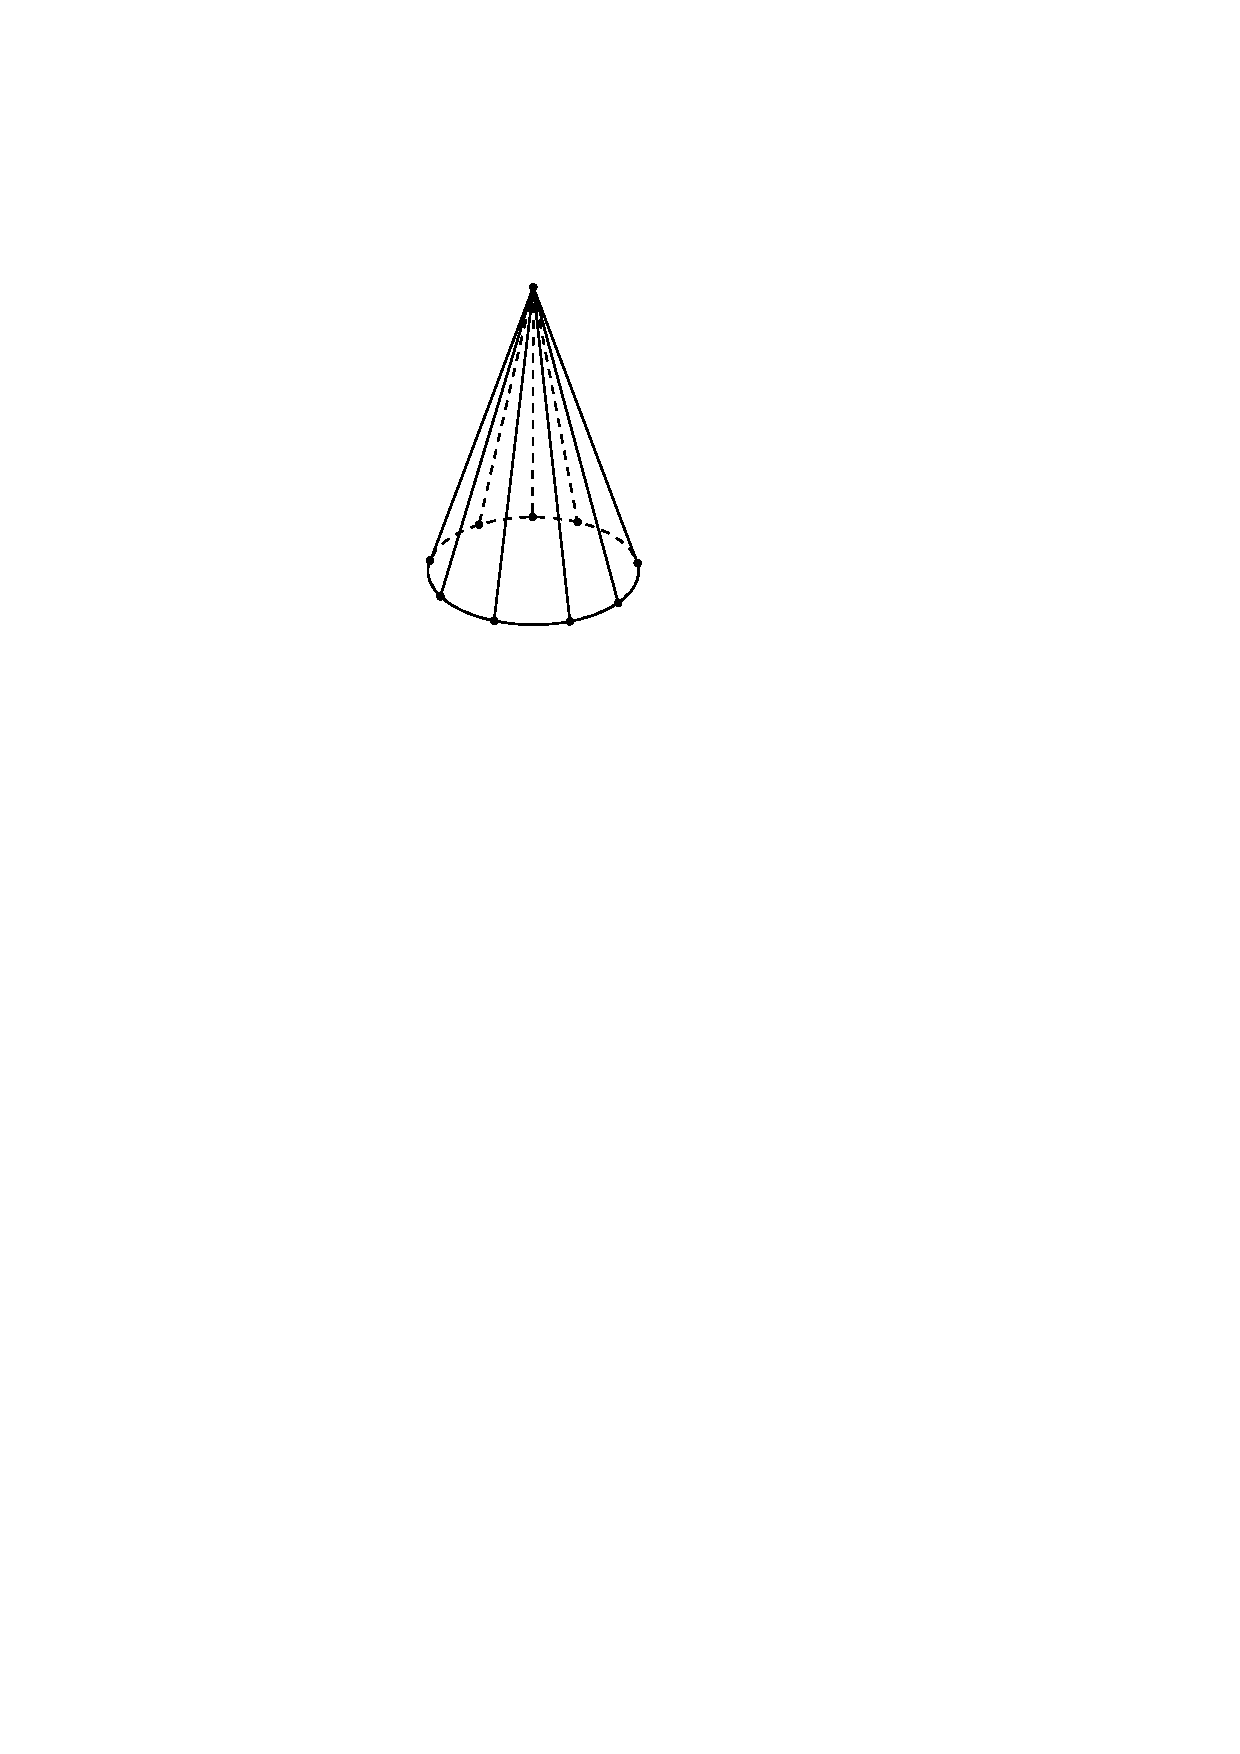
\includegraphics[width=.15\linewidth]{figs/diamond}\hspace{2cm}
    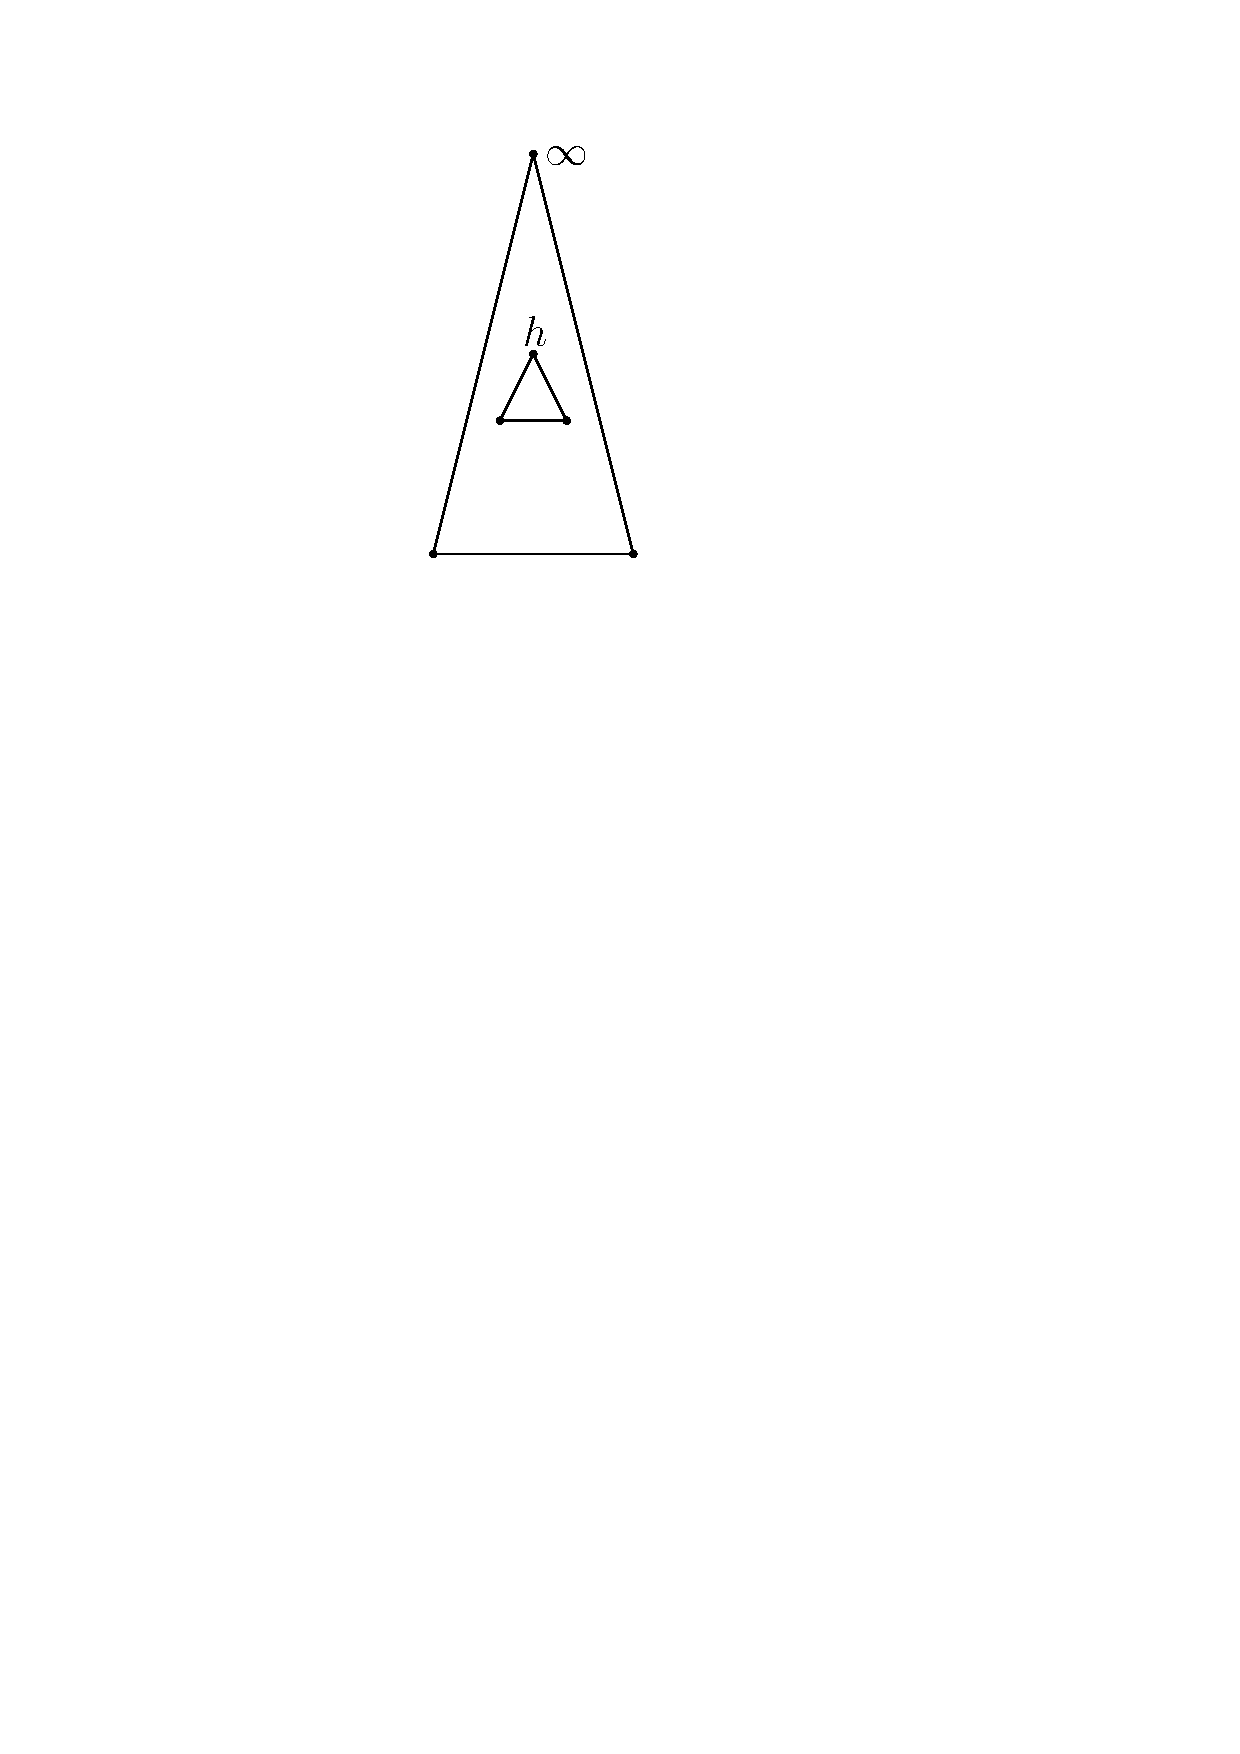
\includegraphics[width=.125\linewidth]{figs/topView}\hspace{2cm}
    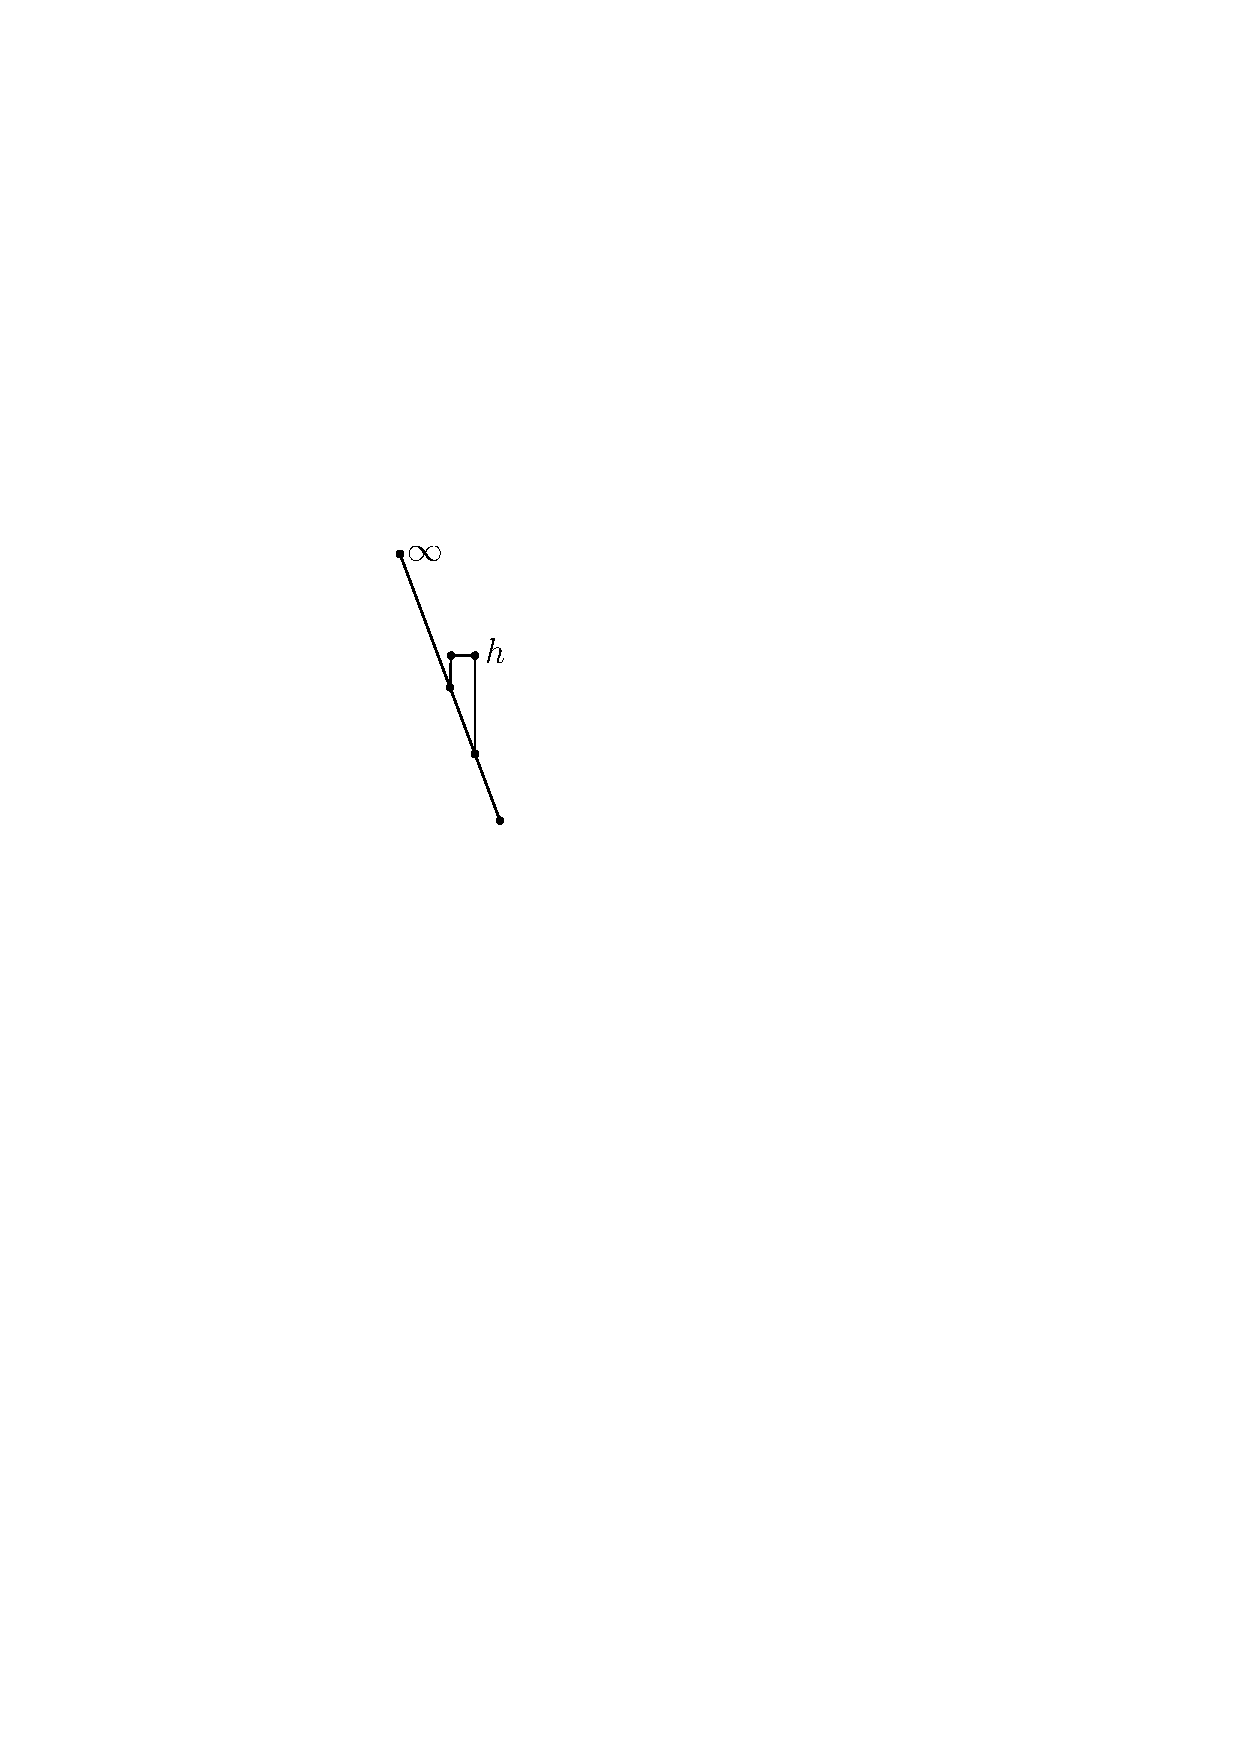
\includegraphics[width=.095\linewidth]{figs/sideView}
    \caption{From left to right: the cone portion of a diamond; the top down view and then the side view of a cone face with a platform added.}
    \label{fig:diamond}
\end{figure}

\begin{lemma}
\label{lem:pathDecomp}
Let $T$ be a merge tree, $P = P(T)$ any path decomposition of $T$, and $\pathTree$ the corresponding path tree.  
Then there are at least $\Pi_{p_i\in P} |p_i|!$ different 2-manifolds with an equivalent path tree.
\end{lemma}
\begin{proof}
 We describe a simple input mesh, with heights specified for all vertices except for the saddles.  The main idea is that 
 this mesh will be flexible enough to allow almost any assignment of heights to the saddles, thus defining a class of merge trees 
 whose size is that described in the lemma statement.
 
 First, we describe the basic building block of this input mesh, which roughly speaking corresponds to a fixed path $p\in P$.  
 Specifically, we say a \emph{diamond} of size $m$ is the following mesh.  To start, construct a cycle 
 of length $m$, where the height of the $i$th vertex in the cycle is say $i/2m$.  Next, create an apex vertex at height 
 $\infty$ (or any appropriately large finite height), and add an edge between this vertex and each vertex in the cycle.  At this point 
 we have built an upside down cone with $m$ triangular faces (see \Fig{diamond}). To make this cone a closed surface we add a triangular cap at the bottom. 
 Specifically, add a $3$ cycle of vertices at heights $0$, $1/20m$, and $1/10m$, and connect each vertex of this $3$-cycle to an arbitrary distinct 
 vertex on the $m$ cycle (with matching cyclic ordering), and triangulate all remaining faces.  For consistency, if the size $m$ is $\leq 3$, the diamond 
 will be just a tetrahedron.
 
 Now above each face of the cone of the diamond, we will create a triangular ``platform'', which will act as the location to glue on other (shrunken) diamonds, 
 and whose highest point of connection to the face below will be a saddle vertex.  Specifically the heights of the vertices of the triangle will be $h$, $h-\eps$, and $h-2\eps$, where 
 $h$ is some unspecified height value.  This near horizontal platform is then connected to its respective face with vertical edges down to the face. See \Fig{diamond}.
 %
 %The vertex at height $h$ will lie in the plane of the respective face of the cone, and the other two will lie above the face, 
 %with edges connecting down to the face, hence creating an actual ``platform''.
 
 At this point we can construct the entire input mesh, by gluing together diamonds.  Specifically, for each path $p_i\in P$ we create a diamond of size $p_i$.
 Now we glue together diamonds of different paths in the same way the paths are connected in $\pathTree$.  Specially, for two paths $p,q\in P$ where 
 $p$ is the parent of $q$ in $\pathTree$, we glue the bottom triangular cap of the diamond for $q$ onto the triangular ``platform'' of some face of the diamond for $p$.
 (Naturally for this construction to work, diamonds for a given path will be scaled down relative to the size of the diamond of their parent).
 
 Observe now that the only saddle points in this construction are the highest connecting point on a face of an edge from the platform above.  Moreover, the only maxima are the apexes of the 
 diamonds, and there is exactly one minima corresponding to the bottom cap of the diamond representing the root of $\pathTree$.  Therefore, the saddles on a given 
 diamond will appear contiguously on a root to leaf path in the merge tree of the mesh, where the leaf corresponds to the maxima of the diamond 
 (since all these saddles have a direct line of sight to this apex).  In particular, 
 this implies that, regardless of the heights assigned to the platforms, the merge tree of this mesh has a path decomposition whose corresponding path 
 tree is equivalent to $\pathTree$.  
 
 Now there is a valid instantiation of this described mesh for any relative ordering of the heights of the saddles on a given diamond.  In particular, 
 there are $|p|!$ possible orderings of the heights of the saddles on the diamond for $p$, and hence $\Pi_{p_i\in P} |p_i|!$ possible instantiations of 
 the mesh overall.  Also, each one of these instantiations will result in a different merge.  Specifically, a permutation of the heights on a given diamond 
 corresponds to a permutation of the vertices along a path in $P$, as by construction all saddles on a given diamond will appear in sorted order in the merge tree.
\end{proof}



\begin{corollary}
 Let $A(S)$ be any algorithm to compute the merge tree of any input surface $S$ (whose contour tree is a merge tree).  
 Then the running time of $A(S)$ is $\Omega(f_{path}(P))=\Omega(\sum_{p_i\in P} |p_i|\log|p_i|)$ where $P$ is any path decomposition of the 
 merge tree of $S$.
\end{corollary}
\begin{proof}
 Given an input surface $S$ whose merge tree has a particular path decomposition $P$, by the above lemma, there are $\Pi_{p_i\in P} |p_i|!$ other surfaces 
 with distinct merge trees, all of which have a path tree equivalent to $\pathTree$.  Therefore, any algorithm which computes the merge tree must distinguish between 
 these possibilities, and therefore its corresponding decision tree must have $\Pi_{p_i\in P} |p_i|!$ leaves.  Hence by Stirling's approximation, 
 this decision tree must have depth $\Omega(\sum_{p_i\in P} |p_i|\log|p_i|)$.
\end{proof}





\subsection{Upper Bound by Path Decomposition}
\Ben{This section is a work in progress.}

From the previous section we now have a lower bound of $\Omega(f_{path}(P))$ for computing the merge tree in terms of any path decomposition $P$. 
We now show that the running time of our algorithm for computing the merge tree is upper bounded by this expression for a specific path decomposition, 
which we will call the maximum path decomposition (defined below).
Specifically, for a given valid coloring $\chi$ of a tree $T$, we will prove that for the maximum path decomposition $f_{alg}(\chi(T)) = O(f_{path}(P(T)))$. 
%using the observations about path decompositions from 
%\Sec{background}, which will then imply $f_{alg}(\chi(T)) = \Theta(f_{path}(P(T)))$.

\subsubsection{Heavy and light paths}

Before describing the maximum path decomposition, we introduce the notion of heavy and light paths 
(which will help motivate what the decomposition should be).

Recall we are ultimately trying to show $f_{alg}(\chi(T)) = O(f_{path}(P(T)))$ for some path decomposition $P=P(T)$, 
or more specifically $\sum_{v\in T} \log |H_v| = O(\sum_{p\in P} |p| \log |p|)$.  In particular, if we could 
show for each path $p\in P$ that $\sum_{v\in p} \log |H_v|= |p|\log|p|$ then we would be done.
In other words we can think of each path as having a budget of $|p|\log|p|$, and ideally the budget 
of each path will pay for the algorithm's cost due to this path.  This is too good to hope for, so instead 
we will divide paths into two categories, called heavy and light, which we show below in \Lem{pathBounds} roughly corresponds 
to whether a path can pay for itself or not.

\begin{definition}
 Let T be a binary tree and let $\chi(T)$ and $P(T)$ be a valid coloring and path decomposition of $T$, respectively.  
 For $p\in P(T)$, we say that $p$ is \emph{light} if $|p| < \sqrt{|H_{r_p}|}/100$, and we say it is \emph{heavy} otherwise.
\end{definition}

\begin{observation}
\label{obs:decrease}
 Let $v$ be a vertex in $T$ and let $w$ be its parent.  Then $|H_w| \geq |H_v| -1$, as $L(T_v) \subseteq L(T_w)$ and the path from 
 $w$ to the root has one less vertex than the path from $v$ to the root.
 
 In particular, we have the following more general property.
 Let $v$ and $u$ be any two vertices in the same root to leaf path of $T$, such that $u$ is lower than $v$.  
 Then $|H_v| \leq |H_u| + d(u,v)$. 
\end{observation}

The following lemma demonstrates that heavy paths can ``pay'' for themselves.

\begin{lemma}
\label{lem:pathBounds}
 Let T be a binary tree and let $\chi(T)$ and $P(T)$ be a valid coloring and path decomposition of $T$, respectively.
 Then, 
 \begin{compactenum}
  \item for any heavy path $p\in P(T)$, $\sum_{v\in p} \log |H_v| = O(|p| \log |p|)$.
  \item for any light path $p\in P(T)$, $\sum_{v\in p} \log |H_v| = O(|p| \log |H_{r_p}|)$.
 \end{compactenum}
\end{lemma}
\begin{proof}
 By $\Obs{decrease}$ we know that for any vertex $v\in p$, $|H_v|\leq |H_{r_p}| + |p|$ (as $r_p$ lies below $v$ on $p$).
 As such, 
 \[
 \sum_{v\in p} \log |H_v| \leq \sum_{v\in p} \log(|H_{r_p}| + |p|)  = |p| \log (|H_{r_p}| + |p|).
 \]
 If $p$ is a heavy path then $|p| \log (|H_{r_p}| + |p|) = O(|p| \log |p|)$, and if $p$ is light then 
 $|p| \log (|H_{r_p}| + |p|) = O(|p| \log |H_{r_p}| )$.
\end{proof}

We are now ready to define the maximum path decomposition, which will allow us to recharge the light paths to heavy paths.


\subsubsection{The decomposition and its main property}

\begin{definition}
 Let $\chi(T)$ be a valid coloring of a binary tree $T$.  We define a set of disjoint paths over the vertices of 
 $T$ as follows.  For each internal vertex $v\in T$ add the edge from $v$ to $\arg \max_{v_l, v_r} \{|H_{v_l}|, |H_{v_r}|\}$ 
 where $v_l$ and $v_r$ are the children of $v$ (if $|H_{v_l}|=|H_{v_r}|$ then pick one arbitrarily).
 The corresponding collection of paths that all such edges correspond to is a path decomposition of $T$, which 
 we refer to as a \emph{maximum} path decomposition, and is denoted by $\mathcal{P}(T)$.  
\end{definition}

We now prove that in a maximum path decomposition, when going between adjacent light paths, the heap size decreases by a constant fraction.

\begin{lemma}
\label{lem:geometric}
 Let $p$ and $q$ be two light paths such that $p$ is the parent of $q$ in the path tree $\pathTreeA$.  
 Then $|H_q|\leq \frac{3}{5} |H_p|$, where $H_p$ and $H_q$ are the heaps at the roots of $p$ and $q$, respectively. 
\end{lemma}
\begin{proof}
 Let $w$ be the vertex in the path $p$ to which the root of the path $q$ is adjacent to in $T$, 
 i.e. $w$ is the parent of $r_q$ in $T$.  Let $c$ be the other child of $w$, which lies in $p$.
 As $\mathcal{P}(T)$ is a maximum path decomposition of $T$ and $c$ rather than $r_q$ is in 
 the same path as $w$, we have $|H_q|\leq |H_c|$.  Therefore, $|H_w|\geq |H_q|+|H_c|-1\geq 2|H_q|-1$. 
 Therefore, by \Obs{decrease}, $|H_p|+ d(r_p, w) \geq |H_w|\geq 2|H_q|-1$.  
 Since $p$ is a light path, $d(r_p, w)\leq \sqrt{|H_p|}/100$ and so we have $|H_p|+\sqrt{|H_p|}/100\geq 2|H_q|-1$.
 Assuming $|H_p|>11$ (and we can safely assume $|H_p|$ is bigger than any constant), this yields $\frac{3}{5} |H_p| \geq |H_q|$
\end{proof}

Naturally, this geometric series behavior can be extended to more than two adjacent light paths, thus motivating 
the following definition.

\begin{definition}
 Let $p$ be a path in a path decomposition $P(T)$, whose corresponding path tree is $\pathTree$.
 Call a light path $q\in P(T)$ light reachable from $p$ if the path from $q$ to $p$ in $\pathTree$ 
 contains only vertices which correspond to light paths.  Call the subtree of $\pathTree$ consisting 
 of all light reachable paths from $p$ the \emph{light path tree} of $p$, and denote is $\mathcal{L}(p)$.
\end{definition}

In the following subsection we show how to exploit this geometric series behavior in light path trees.


\subsubsection{An asymptotically equivalent weight function}
Let $\mathcal{L} = \mathcal{L}(r)$ be a light path tree of some light path $r$ in a maximum path decomposition $\mathcal{P}(T)$.
The intuitive idea is that due to the geometric decreasing behavior of light path trees described in the previous subsection, 
one can show that for the entire light path tree our algorithm pays roughly the cost due to the root path $r$.  This argument 
is hard to make directly, so instead we define an alternative quantity for which we can make the argument.
Specifically, we now define a weight function $w(v)$ for all $v\in \mathcal{L}$, and show that $w(v)=\Theta(|H_v|)$.  

For a path $v\in \mathcal{L}$, let $H_v$ denote the heap at the root of $v$, and let $H_{v_f}$ denote the heap 
at the leaf of $v$.  Let $S_l(v)$ (resp. $S_h(v)$) be the subset of light (resp. heavy) paths adjacent to $v$ in $\mathcal{L}$.

We want to understand how the heap size changes as we move around the paths in $\mathcal{L}$.  Specifically, there are 
three places the vertices in the heap along a light path can come from; adjacent light paths, adjacent heavy paths, and the initial heap at the leaf of the path.  
Given this observation we now define a weight function which upper bounds the size of the heap at the root of any path in $\mathcal{L}$.

First, for all $v\in \mathcal{L}$ we define the local cost function $c(v) = H_{v_f}+\sum_{i\in S_h(v)} H_i$, this is the addition to the heap at $v$ which 
was not already charged to descendant light paths.  We now define a weighted version of $\mathcal{L}$ based on these costs.  
To do so, we first we augment $\mathcal{L}$ by attaching one 
leaf to each vertex in $\mathcal{L}$.  Now for each newly created leaf (which are the only leaves now) assign the cost 
$c(v)$ defined above, where $v$ is that leaf's corresponding parent.  
Now we can define a weight function $w(u)$ over any node $u$ in the tree, which is defined to be the total cost of all leaves in its subtree.   
To simplify notation, we now use $\mathcal{L}$ to refer to this new weighted tree (rather than its unweighted counterpart).

As the weight $w(v)$ includes the sizes of the heaps of all contributing heavy paths and leaves in the subtree rooted at $v$, we have the following.

\begin{claim}
For any $v\in \mathcal{L}$, $w(v)\geq |H_v|$.
\end{claim}

%Let $W= \sum_{v\in \mathcal{L}} w(v) \geq \sum_{v\in \mathcal{L}} |H_v|$.  
%Suppose we could show that conversely $W=O(H_r)$.  Then we would have 
%$\sum_{v\in \mathcal{L}} H_v = O(H_r)$, which was our original goal.  
%So proving $W=O(H_r)$ is now our new goal.

We now would like to show conversely that $w(v)= O(|H_v|)$.  
To do so we first introduce some notation.  
Let $C\subseteq \mathcal{P}$ be the subset of paths that are leaves in $\mathcal{L}$.
For any path $v$, let $\mathcal{L}_v$ (resp. $C_v$) be the subset of paths in $\mathcal{L}$ (resp $C$) 
that are contained in the subtree of $\mathcal{L}$ which is rooted at $v$.

First, observe that $|H_v|\geq w(v)-\sum_{u\in \mathcal{L}_v} |u|$.  
This holds by the same argument as in \Lem{adjacent}, namely, $w(u)$ by definition 
counts all the contributing heavy path heaps and initial leaf heaps that contribute 
to the heap at $v$ and $\sum_{u\in \mathcal{L}_v} |u|$ is an upper bound on the number 
of vertices that could have been removed from one of these heaps before reaching the 
root of $v$ (since a vertex in a heap can only get removed if it appears on one of 
the paths).  

As all paths in $\mathcal{L}$ are light, we thus have the following.

\begin{claim}
$|H_v|\geq w(v)-\sum_{u\in \mathcal{L}_v} \sqrt{|H_u|}/100 \geq w(v)-\sum_{u\in \mathcal{L}_v} \sqrt{w(u)}/100$
\end{claim}

By the above claim, if we can prove $\sum_{u\in \mathcal{L}_v} \sqrt{w(u)}/100 \leq w(v)/c$ for some constant $c>1$, 
then we will have proven that $|H_v| = \Theta(w(v))$.  

Recall that \Lem{geometric} told us that that $|H_{u}|\leq (3/5) |H_{u'}|$, if $u'$ is the parent $u$ in $\mathcal{L}$. 
The following lemma shows that if we had a similar statement in terms of the weights rather than the heap sizes, 
then we get the desired bound on the sum.

\begin{lemma}
\label{lem:distribution}
Let $v$ be a path in $\mathcal{L}$.  Suppose that for any two paths $x,y\in \mathcal{L}_v$ 
such that $y$ is the parent of $x$, $w(x)\leq (4/5) w(y)$.
Then $\sum_{u\in \mathcal{P}_v} \sqrt{w(u)}/100 \leq \sum_{c\in C_v} \sqrt{w(c)}/10$
\end{lemma}

\begin{proof}
The idea is to recursively redistribute the contribution to the sum of each internal vertex to its children, 
until all the weight sits on the leaves.  Specifically, let $v$ be some path in $\mathcal{L}$.  Its 
contribution to the sum is $\sqrt{w(v)}/100$, which we will call the value at $v$.  We redistribute this 
value to its children, in proportion by the weight of each child.  For example, if $v$ has a child $x$ then 
the fraction it gets assigned is $w(x)/w(v)$ (recall that by definition $w(v)$ is the sum of the weights of 
its children and so the total value will get reassigned to the children).

Suppose we keep redistributing the value of $v$ until it reaches the leaves of its subtree in $\mathcal{L}$.  
Let's see how much gets assigned to a given leaf.  Specifically, let $u_0, u_1, \ldots, u_k$ 
be a path in $\mathcal{L}$ (of paths from the set $\mathcal{P}_v$), such that $v=u_0$, $u_{i+1}$ 
is child of $u_i$ for all $i$, and $u_k$ is a leaf of $\mathcal{L}$.  

Then the total value from $u_0$ that ends up at $u_k$ is 
\[
\frac{\sqrt{w(u_0)}}{100} \pth{ \frac{w(u_1)}{w(u_0)} \frac{w(u_2)}{w(u_1)} \cdots \frac{w(u_k)}{w(u_{k-1})} }
= \frac{\sqrt{w(u_0)}}{100} \pth{ \frac{w(u_k)}{w(u_0)} } = \frac{w(u_k)}{100\sqrt{w(u_0)}}
\]

For a given leaf in $\mathcal{L}$, we can calculate the total value reassigned to it from it its ancestors.
Specifically, let $u_0, u_1, u_2, \dots, u_m$ be a root to leaf path in $\mathcal{L}$ 
(i.e. $u_0$ is the root $r$ of $\mathcal{L}$).

By assumption from the lemma statement we have $w(u_{i+1})\leq (4/5) w(u_i)$.  Therefore by the above calculation, 
the total reassigned to $u_m$ is 

\[
 \sum_{i=0}^m \frac{w(u_m)}{100\sqrt{w(u_i)}} \leq \frac{w(u_m)}{100} \sum_{i=0}^m 1 \Big/ \sqrt{\pth{\frac{5}{4}}^iw(u_m)} 
 \leq \frac{\sqrt{w(u_m)}}{100} \sum_{i=0}^{\infty} \pth{\frac{4}{5}}^{i/2} \leq \frac{\sqrt{w(u_m)}}{10}
\]

The claim then follows by summing this quantity over the children of $\mathcal{L}$.
\end{proof}

By combining the above lemma and claim we have the following.

\begin{claim}
For any path $v\in \mathcal{L}$ if it holds that 
$w(x)\leq (4/5) w(y)$ for any two paths $x,y\in \mathcal{L}_v$ such that $y$ is the parent of $x$, then 

\[
|H_v|\geq w(v)-\sum_{u\in \mathcal{L}_v} \sqrt{w(u)}/100 \geq w(v)- \sum_{c\in C_v} \sqrt{w(c)}/10 \geq \frac{4}{5} w(v)
\]
\end{claim}



\begin{lemma}
Let $\mathcal{L}$ be the light path tree of some path $r$.  
Then for any $v\in \mathcal{L}$, we have $|H_v|\geq \frac{4}{5} w(v)$.
\end{lemma}
% \begin{proof}
% We will actually prove the stronger statement that for any $v\in \mathcal{L}$, 
% we have $|H_v|\geq \frac{4}{5} w(v)$ and $w(v)\leq (4/5) w(p)$ where $p$ is the parent 
% of $v$ in $\mathcal{L}$.
% 
% Suppose otherwise, and let $v$ be the lowest path in $\mathcal{L}$ such that this fails 
% (i.e. the statement holds for all descendants of $v$ in $\mathcal{L}$).  Then for any 
% two paths $x,y\in \mathcal{L}_v$ such that $y$ is the parent of $x$, 
% we have that $w(x)\leq (4/5) w(y)$ and so by \Lem{distribution}, $|H_v|\geq \frac{4}{5} w(v)$.
% Combining this fact with \Lem{geometric} gives,
% \[
% w(v) \leq \frac{5}{4}|H_v| \leq \frac{5}{4} \frac{3}{5} |H_p| \leq \frac{3}{4} w(p).
% \]
% 
% \end{proof}
%
\begin{proof}
By the above claim, we know that $|H_v|\geq \frac{4}{5} w(v)$ if it holds that 
$w(x)\leq (4/5) w(y)$ for any two paths $x,y\in \mathcal{L}_v$ such that $y$ is the parent of $x$.
So let $v$ be the lowest path in $\mathcal{L}$ such that this fractional decrease fails to hold, i.e. $w(c)> (4/5) w(v)$ 
where $c$ is a child of $v$ in $\mathcal{L}$, and conversely all vertices in $\mathcal{L}_c$ 
the fractional decrease holds.  As the fractional decrease holds for a paths in $\mathcal{L}_c$, 
we have $|H_c|\geq \frac{4}{5} w(c)$.  Therefore,
\[
w(c) \leq \frac{5}{4}|H_c| \leq \frac{5}{4} \frac{3}{5} |H_v| \leq \frac{3}{4} w(v).
\]
However, this is a contradiction with the assumption $w(c)> (4/5) w(v)$ , and hence the 
fractional decrease always holds implying the claim always holds.
\end{proof}

\begin{corollary}
 Let $\mathcal{L}$ be a light path tree of a light path $r$.  Then for any $v\in \mathcal{L}$, $w(v) = O(|H_v|)$.
\end{corollary}





%
%
% So $w(r)$ upper bound $H_r$, but by how much?  Consider a path $v\in \mathcal{L}$.  
% As we move from the leaf to the root of $v$ we now want to understand 
% how the heap can decreases.  Now the only way a vertex in the heap can leave that 
% heap is if that vertex is one of the vertices we traverse in $v$, i.e. the total 
% loss in vertices from the heap along $v$ is bounded by $|v|$.  
% Therefore, $|H_r|\geq W-\sum_{v\in \mathcal{L}} |v|$.  
% (This is an extension of \Lem{adjacent}, and probably should be merged with it.)
% As $\mathcal{L}$ consists of only light paths we have $|v|\leq \sqrt{|H_v|}/100 \leq \sqrt{w(v)}/100$, 
% and therefore $|H_r|\geq W-\sum_{v\in \mathcal{L}} \sqrt{w(v)}/100$.











\pagebreak
\subsection{Junk, don't read}

\begin{lemma}
 Let $\chi(T)$ be a valid coloring of a tree $T$, and let $\mathcal{P}(T)$ be the corresponding maximum path decomposition.
 Let $p$ be a light path in $\mathcal{P}(T)$ and let $LPT(p)$ be the light path tree of $p$.
 
 Then $\sum_{q\in L(p)} \sum_{v\in q} \log |H_v| = |H_p|\log |H_p|$.
\end{lemma}
\begin{proof}UNDER CONSTRUCTION / NOTES:

 Claim: Let $q$ be some path of depth $i$ in $LPT(p)$, and let $H_q$ be the heap at the root of this path.
 Then $|H_q|< |H_p|/c^i$ for some constant $c>1$.  This should follow from using a maximum path decomposition.
 
 This claim would imply the depth of the tree is $O(\log |H_p|)$ and the total number of paths in the tree is $O(|H_p|)$, 
 thought I am not sure if either of these statements are useful.
\end{proof}



%%%%%%%%%%%%%%%%%%%%%%%%%%%%%%%%%%%%%%%%%%%%%%%%%%%%%%%
%%%%%%%%%%%%%%%%%%%%%%%%%%%%%%%%%%%%%%%%%%%%%%%%%%%%%%%
\subsection{More Junk}

The following can be viewed as stronger version of \Lem{adjacent}, which is possible as the path is now assumed to be maximum.

\begin{lemma}
 Let $\chi(T)$ be a valid coloring of a tree $T$, and let $\mathcal{P}(T)$ be the corresponding maximum path decomposition.
 Let $p$ be a light path in $\mathcal{P}(T)$ and let $\{q_1, \dots q_k\}$ be the set of all light paths adjacent to $p$.
 
 For $1\leq i\leq k$ let $r_i = r_{q_i}$ and let $H_i = H_{r_i}$.
  Then $\sum_{i=1}^k |H_i| \leq |H_p|/c$ for some constant $c>1$, where $H_p = H_{r_p}$.
\end{lemma}


% \begin{proof}UNDER CONSTRUCTION: 
% For simplicity, let $H_{k+1}$ denote the heap at the leaf vertex of $p$.  As the $H_k+1$ is disjoing from all other $H_{i}$, \Lem{adjacent} implies that 
% $H_p > \sum_{j=1}^{k+1} H_i - |p|$.  
% 
% Let $x$ be the largest index such that $H_x > H_p / 3$.
% By the above observation and since $p$ is a light path we have 
% \[
%  H_p > \sum_{j=1}^{k} H_i + H_{k+1} - |p|
% \] 
% \end{proof}







\bibliographystyle{alpha}
\bibliography{contour}

\end{document}
